% error_floorplan_ab.tex — HAND-WRITTEN assembly: rows (a) and (b) only.
% The panel files it \input are still generated by `make floorplan`; only
% this table is authored. Row (c) (median rotation per station) is omitted
% deliberately: the paper reports that the BlobBoard median rotation error
% sits within a factor of two of the hand-eye calibration residual, so a
% per-station median-rotation comparison is not resolvable by the ground
% truth. `make floorplan` regenerates error_floorplan_table.tex, NOT this.
% class-agnostic: manual (a)/(b)/(c) caption lines, NO subcaption
% (bmvc2k's caption machinery mis-numbers subcaption subfigures)
% requires: \usepackage{graphicx,pgfplots} \pgfplotsset{compat=1.18}
\providecommand{\fpscale}{1}\renewcommand{\fpscale}{0.42}   % fan geometry scale (fonts unaffected)
\setlength{\tabcolsep}{3pt}
\centering
\begin{tabular}{@{}ccc l@{}}
\textbf{BlobBoards} & \textbf{AprilTag} & \textbf{ArUco} & \\[2pt]
% floorplan fan: BlobBoards / det — generated, edit freely
\providecommand{\fpscale}{1}
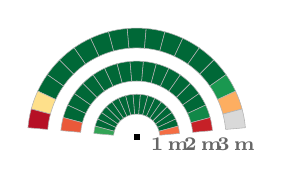
\begin{tikzpicture}[x=\fpscale cm, y=\fpscale cm, baseline=(current bounding box.north)]
  \fill[fill={rgb,1:red,0.0;green,0.408;blue,0.216}, draw=black!30, line width=0.2pt] (95.0:0.7) arc[start angle=95.0, end angle=85.0, radius=0.7] -- (85.0:1.3) arc[start angle=85.0, end angle=95.0, radius=1.3] -- cycle;
  \fill[fill={rgb,1:red,0.0;green,0.408;blue,0.216}, draw=black!30, line width=0.2pt] (105.0:0.7) arc[start angle=105.0, end angle=95.0, radius=0.7] -- (95.0:1.3) arc[start angle=95.0, end angle=105.0, radius=1.3] -- cycle;
  \fill[fill={rgb,1:red,0.0;green,0.408;blue,0.216}, draw=black!30, line width=0.2pt] (115.0:0.7) arc[start angle=115.0, end angle=105.0, radius=0.7] -- (105.0:1.3) arc[start angle=105.0, end angle=115.0, radius=1.3] -- cycle;
  \fill[fill={rgb,1:red,0.0;green,0.408;blue,0.216}, draw=black!30, line width=0.2pt] (125.0:0.7) arc[start angle=125.0, end angle=115.0, radius=0.7] -- (115.0:1.3) arc[start angle=115.0, end angle=125.0, radius=1.3] -- cycle;
  \fill[fill={rgb,1:red,0.0;green,0.408;blue,0.216}, draw=black!30, line width=0.2pt] (135.0:0.7) arc[start angle=135.0, end angle=125.0, radius=0.7] -- (125.0:1.3) arc[start angle=125.0, end angle=135.0, radius=1.3] -- cycle;
  \fill[fill={rgb,1:red,0.0;green,0.408;blue,0.216}, draw=black!30, line width=0.2pt] (145.0:0.7) arc[start angle=145.0, end angle=135.0, radius=0.7] -- (135.0:1.3) arc[start angle=135.0, end angle=145.0, radius=1.3] -- cycle;
  \fill[fill={rgb,1:red,0.0;green,0.408;blue,0.216}, draw=black!30, line width=0.2pt] (155.0:0.7) arc[start angle=155.0, end angle=145.0, radius=0.7] -- (145.0:1.3) arc[start angle=145.0, end angle=155.0, radius=1.3] -- cycle;
  \fill[fill={rgb,1:red,0.0;green,0.408;blue,0.216}, draw=black!30, line width=0.2pt] (165.0:0.7) arc[start angle=165.0, end angle=155.0, radius=0.7] -- (155.0:1.3) arc[start angle=155.0, end angle=165.0, radius=1.3] -- cycle;
  \fill[fill={rgb,1:red,0.2013;green,0.6443;blue,0.3387}, draw=black!30, line width=0.2pt] (175.0:0.7) arc[start angle=175.0, end angle=165.0, radius=0.7] -- (165.0:1.3) arc[start angle=165.0, end angle=175.0, radius=1.3] -- cycle;
  \fill[fill={rgb,1:red,0.0;green,0.408;blue,0.216}, draw=black!30, line width=0.2pt] (85.0:0.7) arc[start angle=85.0, end angle=75.0, radius=0.7] -- (75.0:1.3) arc[start angle=75.0, end angle=85.0, radius=1.3] -- cycle;
  \fill[fill={rgb,1:red,0.0;green,0.408;blue,0.216}, draw=black!30, line width=0.2pt] (75.0:0.7) arc[start angle=75.0, end angle=65.0, radius=0.7] -- (65.0:1.3) arc[start angle=65.0, end angle=75.0, radius=1.3] -- cycle;
  \fill[fill={rgb,1:red,0.0;green,0.408;blue,0.216}, draw=black!30, line width=0.2pt] (65.0:0.7) arc[start angle=65.0, end angle=55.0, radius=0.7] -- (55.0:1.3) arc[start angle=55.0, end angle=65.0, radius=1.3] -- cycle;
  \fill[fill={rgb,1:red,0.0;green,0.408;blue,0.216}, draw=black!30, line width=0.2pt] (55.0:0.7) arc[start angle=55.0, end angle=45.0, radius=0.7] -- (45.0:1.3) arc[start angle=45.0, end angle=55.0, radius=1.3] -- cycle;
  \fill[fill={rgb,1:red,0.0;green,0.408;blue,0.216}, draw=black!30, line width=0.2pt] (45.0:0.7) arc[start angle=45.0, end angle=35.0, radius=0.7] -- (35.0:1.3) arc[start angle=35.0, end angle=45.0, radius=1.3] -- cycle;
  \fill[fill={rgb,1:red,0.0;green,0.408;blue,0.216}, draw=black!30, line width=0.2pt] (35.0:0.7) arc[start angle=35.0, end angle=25.0, radius=0.7] -- (25.0:1.3) arc[start angle=25.0, end angle=35.0, radius=1.3] -- cycle;
  \fill[fill={rgb,1:red,0.0;green,0.408;blue,0.216}, draw=black!30, line width=0.2pt] (25.0:0.7) arc[start angle=25.0, end angle=15.0, radius=0.7] -- (15.0:1.3) arc[start angle=15.0, end angle=25.0, radius=1.3] -- cycle;
  \fill[fill={rgb,1:red,0.957;green,0.427;blue,0.263}, draw=black!30, line width=0.2pt] (15.0:0.7) arc[start angle=15.0, end angle=5.0, radius=0.7] -- (5.0:1.3) arc[start angle=5.0, end angle=15.0, radius=1.3] -- cycle;
  \fill[fill={rgb,1:red,0.0;green,0.408;blue,0.216}, draw=black!30, line width=0.2pt] (105.0:1.7) arc[start angle=105.0, end angle=95.0, radius=1.7] -- (95.0:2.3) arc[start angle=95.0, end angle=105.0, radius=2.3] -- cycle;
  \fill[fill={rgb,1:red,0.0;green,0.408;blue,0.216}, draw=black!30, line width=0.2pt] (85.0:1.7) arc[start angle=85.0, end angle=75.0, radius=1.7] -- (75.0:2.3) arc[start angle=75.0, end angle=85.0, radius=2.3] -- cycle;
  \fill[fill={rgb,1:red,0.0;green,0.408;blue,0.216}, draw=black!30, line width=0.2pt] (115.0:1.7) arc[start angle=115.0, end angle=105.0, radius=1.7] -- (105.0:2.3) arc[start angle=105.0, end angle=115.0, radius=2.3] -- cycle;
  \fill[fill={rgb,1:red,0.0;green,0.408;blue,0.216}, draw=black!30, line width=0.2pt] (125.0:1.7) arc[start angle=125.0, end angle=115.0, radius=1.7] -- (115.0:2.3) arc[start angle=115.0, end angle=125.0, radius=2.3] -- cycle;
  \fill[fill={rgb,1:red,0.0;green,0.408;blue,0.216}, draw=black!30, line width=0.2pt] (135.0:1.7) arc[start angle=135.0, end angle=125.0, radius=1.7] -- (125.0:2.3) arc[start angle=125.0, end angle=135.0, radius=2.3] -- cycle;
  \fill[fill={rgb,1:red,0.0;green,0.408;blue,0.216}, draw=black!30, line width=0.2pt] (145.0:1.7) arc[start angle=145.0, end angle=135.0, radius=1.7] -- (135.0:2.3) arc[start angle=135.0, end angle=145.0, radius=2.3] -- cycle;
  \fill[fill={rgb,1:red,0.0;green,0.408;blue,0.216}, draw=black!30, line width=0.2pt] (155.0:1.7) arc[start angle=155.0, end angle=145.0, radius=1.7] -- (145.0:2.3) arc[start angle=145.0, end angle=155.0, radius=2.3] -- cycle;
  \fill[fill={rgb,1:red,0.0;green,0.408;blue,0.216}, draw=black!30, line width=0.2pt] (165.0:1.7) arc[start angle=165.0, end angle=155.0, radius=1.7] -- (155.0:2.3) arc[start angle=155.0, end angle=165.0, radius=2.3] -- cycle;
  \fill[fill={rgb,1:red,0.919;green,0.3473;blue,0.2263}, draw=black!30, line width=0.2pt] (175.0:1.7) arc[start angle=175.0, end angle=165.0, radius=1.7] -- (165.0:2.3) arc[start angle=165.0, end angle=175.0, radius=2.3] -- cycle;
  \fill[fill={rgb,1:red,0.0;green,0.408;blue,0.216}, draw=black!30, line width=0.2pt] (95.0:1.7) arc[start angle=95.0, end angle=85.0, radius=1.7] -- (85.0:2.3) arc[start angle=85.0, end angle=95.0, radius=2.3] -- cycle;
  \fill[fill={rgb,1:red,0.0;green,0.408;blue,0.216}, draw=black!30, line width=0.2pt] (75.0:1.7) arc[start angle=75.0, end angle=65.0, radius=1.7] -- (65.0:2.3) arc[start angle=65.0, end angle=75.0, radius=2.3] -- cycle;
  \fill[fill={rgb,1:red,0.0;green,0.408;blue,0.216}, draw=black!30, line width=0.2pt] (65.0:1.7) arc[start angle=65.0, end angle=55.0, radius=1.7] -- (55.0:2.3) arc[start angle=55.0, end angle=65.0, radius=2.3] -- cycle;
  \fill[fill={rgb,1:red,0.0;green,0.408;blue,0.216}, draw=black!30, line width=0.2pt] (55.0:1.7) arc[start angle=55.0, end angle=45.0, radius=1.7] -- (45.0:2.3) arc[start angle=45.0, end angle=55.0, radius=2.3] -- cycle;
  \fill[fill={rgb,1:red,0.0;green,0.408;blue,0.216}, draw=black!30, line width=0.2pt] (45.0:1.7) arc[start angle=45.0, end angle=35.0, radius=1.7] -- (35.0:2.3) arc[start angle=35.0, end angle=45.0, radius=2.3] -- cycle;
  \fill[fill={rgb,1:red,0.0;green,0.408;blue,0.216}, draw=black!30, line width=0.2pt] (35.0:1.7) arc[start angle=35.0, end angle=25.0, radius=1.7] -- (25.0:2.3) arc[start angle=25.0, end angle=35.0, radius=2.3] -- cycle;
  \fill[fill={rgb,1:red,0.068;green,0.5333;blue,0.2813}, draw=black!30, line width=0.2pt] (25.0:1.7) arc[start angle=25.0, end angle=15.0, radius=1.7] -- (15.0:2.3) arc[start angle=15.0, end angle=25.0, radius=2.3] -- cycle;
  \fill[fill={rgb,1:red,0.7777;green,0.1253;blue,0.1517}, draw=black!30, line width=0.2pt] (15.0:1.7) arc[start angle=15.0, end angle=5.0, radius=1.7] -- (5.0:2.3) arc[start angle=5.0, end angle=15.0, radius=2.3] -- cycle;
  \fill[fill={rgb,1:red,0.0;green,0.408;blue,0.216}, draw=black!30, line width=0.2pt] (95.0:2.7) arc[start angle=95.0, end angle=85.0, radius=2.7] -- (85.0:3.3) arc[start angle=85.0, end angle=95.0, radius=3.3] -- cycle;
  \fill[fill={rgb,1:red,0.0;green,0.408;blue,0.216}, draw=black!30, line width=0.2pt] (105.0:2.7) arc[start angle=105.0, end angle=95.0, radius=2.7] -- (95.0:3.3) arc[start angle=95.0, end angle=105.0, radius=3.3] -- cycle;
  \fill[fill={rgb,1:red,0.0;green,0.408;blue,0.216}, draw=black!30, line width=0.2pt] (115.0:2.7) arc[start angle=115.0, end angle=105.0, radius=2.7] -- (105.0:3.3) arc[start angle=105.0, end angle=115.0, radius=3.3] -- cycle;
  \fill[fill={rgb,1:red,0.0;green,0.408;blue,0.216}, draw=black!30, line width=0.2pt] (125.0:2.7) arc[start angle=125.0, end angle=115.0, radius=2.7] -- (115.0:3.3) arc[start angle=115.0, end angle=125.0, radius=3.3] -- cycle;
  \fill[fill={rgb,1:red,0.0;green,0.408;blue,0.216}, draw=black!30, line width=0.2pt] (135.0:2.7) arc[start angle=135.0, end angle=125.0, radius=2.7] -- (125.0:3.3) arc[start angle=125.0, end angle=135.0, radius=3.3] -- cycle;
  \fill[fill={rgb,1:red,0.0;green,0.408;blue,0.216}, draw=black!30, line width=0.2pt] (145.0:2.7) arc[start angle=145.0, end angle=135.0, radius=2.7] -- (135.0:3.3) arc[start angle=135.0, end angle=145.0, radius=3.3] -- cycle;
  \fill[fill={rgb,1:red,0.0;green,0.408;blue,0.216}, draw=black!30, line width=0.2pt] (155.0:2.7) arc[start angle=155.0, end angle=145.0, radius=2.7] -- (145.0:3.3) arc[start angle=145.0, end angle=155.0, radius=3.3] -- cycle;
  \fill[fill={rgb,1:red,0.996;green,0.878;blue,0.545}, draw=black!30, line width=0.2pt] (165.0:2.7) arc[start angle=165.0, end angle=155.0, radius=2.7] -- (155.0:3.3) arc[start angle=155.0, end angle=165.0, radius=3.3] -- cycle;
  \fill[fill={rgb,1:red,0.7123;green,0.0627;blue,0.1503}, draw=black!30, line width=0.2pt] (175.0:2.7) arc[start angle=175.0, end angle=165.0, radius=2.7] -- (165.0:3.3) arc[start angle=165.0, end angle=175.0, radius=3.3] -- cycle;
  \fill[fill={rgb,1:red,0.0;green,0.408;blue,0.216}, draw=black!30, line width=0.2pt] (85.0:2.7) arc[start angle=85.0, end angle=75.0, radius=2.7] -- (75.0:3.3) arc[start angle=75.0, end angle=85.0, radius=3.3] -- cycle;
  \fill[fill={rgb,1:red,0.0;green,0.408;blue,0.216}, draw=black!30, line width=0.2pt] (75.0:2.7) arc[start angle=75.0, end angle=65.0, radius=2.7] -- (65.0:3.3) arc[start angle=65.0, end angle=75.0, radius=3.3] -- cycle;
  \fill[fill={rgb,1:red,0.0;green,0.408;blue,0.216}, draw=black!30, line width=0.2pt] (65.0:2.7) arc[start angle=65.0, end angle=55.0, radius=2.7] -- (55.0:3.3) arc[start angle=55.0, end angle=65.0, radius=3.3] -- cycle;
  \fill[fill={rgb,1:red,0.0;green,0.408;blue,0.216}, draw=black!30, line width=0.2pt] (55.0:2.7) arc[start angle=55.0, end angle=45.0, radius=2.7] -- (45.0:3.3) arc[start angle=45.0, end angle=55.0, radius=3.3] -- cycle;
  \fill[fill={rgb,1:red,0.0;green,0.408;blue,0.216}, draw=black!30, line width=0.2pt] (45.0:2.7) arc[start angle=45.0, end angle=35.0, radius=2.7] -- (35.0:3.3) arc[start angle=35.0, end angle=45.0, radius=3.3] -- cycle;
  \fill[fill={rgb,1:red,0.102;green,0.596;blue,0.314}, draw=black!30, line width=0.2pt] (35.0:2.7) arc[start angle=35.0, end angle=25.0, radius=2.7] -- (25.0:3.3) arc[start angle=25.0, end angle=35.0, radius=3.3] -- cycle;
  \fill[fill={rgb,1:red,0.992;green,0.682;blue,0.38}, draw=black!30, line width=0.2pt] (25.0:2.7) arc[start angle=25.0, end angle=15.0, radius=2.7] -- (15.0:3.3) arc[start angle=15.0, end angle=25.0, radius=3.3] -- cycle;
  \fill[fill=gray!30, draw=black!30, line width=0.2pt] (15.0:2.7) arc[start angle=15.0, end angle=5.0, radius=2.7] -- (5.0:3.3) arc[start angle=5.0, end angle=15.0, radius=3.3] -- cycle;
  \fill[black] (-0.09, -0.09) rectangle (0.09, 0.09);
  \node[font=\scriptsize\bfseries, text=black!60] at (1, -0.22) {1\,m};
  \node[font=\scriptsize\bfseries, text=black!60] at (2, -0.22) {2\,m};
  \node[font=\scriptsize\bfseries, text=black!60] at (3, -0.22) {3\,m};
\end{tikzpicture}
 & % floorplan fan: AprilTag / det — generated, edit freely
\providecommand{\fpscale}{1}
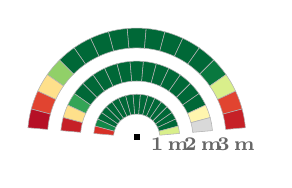
\begin{tikzpicture}[x=\fpscale cm, y=\fpscale cm, baseline=(current bounding box.north)]
  \fill[fill={rgb,1:red,0.0;green,0.408;blue,0.216}, draw=black!30, line width=0.2pt] (95.0:0.7) arc[start angle=95.0, end angle=85.0, radius=0.7] -- (85.0:1.3) arc[start angle=85.0, end angle=95.0, radius=1.3] -- cycle;
  \fill[fill={rgb,1:red,0.0;green,0.408;blue,0.216}, draw=black!30, line width=0.2pt] (105.0:0.7) arc[start angle=105.0, end angle=95.0, radius=0.7] -- (95.0:1.3) arc[start angle=95.0, end angle=105.0, radius=1.3] -- cycle;
  \fill[fill={rgb,1:red,0.0;green,0.408;blue,0.216}, draw=black!30, line width=0.2pt] (115.0:0.7) arc[start angle=115.0, end angle=105.0, radius=0.7] -- (105.0:1.3) arc[start angle=105.0, end angle=115.0, radius=1.3] -- cycle;
  \fill[fill={rgb,1:red,0.0;green,0.408;blue,0.216}, draw=black!30, line width=0.2pt] (125.0:0.7) arc[start angle=125.0, end angle=115.0, radius=0.7] -- (115.0:1.3) arc[start angle=115.0, end angle=125.0, radius=1.3] -- cycle;
  \fill[fill={rgb,1:red,0.0;green,0.408;blue,0.216}, draw=black!30, line width=0.2pt] (135.0:0.7) arc[start angle=135.0, end angle=125.0, radius=0.7] -- (125.0:1.3) arc[start angle=125.0, end angle=135.0, radius=1.3] -- cycle;
  \fill[fill={rgb,1:red,0.0;green,0.408;blue,0.216}, draw=black!30, line width=0.2pt] (145.0:0.7) arc[start angle=145.0, end angle=135.0, radius=0.7] -- (135.0:1.3) arc[start angle=135.0, end angle=145.0, radius=1.3] -- cycle;
  \fill[fill={rgb,1:red,0.0;green,0.408;blue,0.216}, draw=black!30, line width=0.2pt] (155.0:0.7) arc[start angle=155.0, end angle=145.0, radius=0.7] -- (145.0:1.3) arc[start angle=145.0, end angle=155.0, radius=1.3] -- cycle;
  \fill[fill={rgb,1:red,0.068;green,0.5333;blue,0.2813}, draw=black!30, line width=0.2pt] (165.0:0.7) arc[start angle=165.0, end angle=155.0, radius=0.7] -- (155.0:1.3) arc[start angle=155.0, end angle=165.0, radius=1.3] -- cycle;
  \fill[fill={rgb,1:red,0.843;green,0.188;blue,0.153}, draw=black!30, line width=0.2pt] (175.0:0.7) arc[start angle=175.0, end angle=165.0, radius=0.7] -- (165.0:1.3) arc[start angle=165.0, end angle=175.0, radius=1.3] -- cycle;
  \fill[fill={rgb,1:red,0.0;green,0.408;blue,0.216}, draw=black!30, line width=0.2pt] (85.0:0.7) arc[start angle=85.0, end angle=75.0, radius=0.7] -- (75.0:1.3) arc[start angle=75.0, end angle=85.0, radius=1.3] -- cycle;
  \fill[fill={rgb,1:red,0.0;green,0.408;blue,0.216}, draw=black!30, line width=0.2pt] (75.0:0.7) arc[start angle=75.0, end angle=65.0, radius=0.7] -- (65.0:1.3) arc[start angle=65.0, end angle=75.0, radius=1.3] -- cycle;
  \fill[fill={rgb,1:red,0.0;green,0.408;blue,0.216}, draw=black!30, line width=0.2pt] (65.0:0.7) arc[start angle=65.0, end angle=55.0, radius=0.7] -- (55.0:1.3) arc[start angle=55.0, end angle=65.0, radius=1.3] -- cycle;
  \fill[fill={rgb,1:red,0.0;green,0.408;blue,0.216}, draw=black!30, line width=0.2pt] (55.0:0.7) arc[start angle=55.0, end angle=45.0, radius=0.7] -- (45.0:1.3) arc[start angle=45.0, end angle=55.0, radius=1.3] -- cycle;
  \fill[fill={rgb,1:red,0.0;green,0.408;blue,0.216}, draw=black!30, line width=0.2pt] (45.0:0.7) arc[start angle=45.0, end angle=35.0, radius=0.7] -- (35.0:1.3) arc[start angle=35.0, end angle=45.0, radius=1.3] -- cycle;
  \fill[fill={rgb,1:red,0.0;green,0.408;blue,0.216}, draw=black!30, line width=0.2pt] (35.0:0.7) arc[start angle=35.0, end angle=25.0, radius=0.7] -- (25.0:1.3) arc[start angle=25.0, end angle=35.0, radius=1.3] -- cycle;
  \fill[fill={rgb,1:red,0.0;green,0.408;blue,0.216}, draw=black!30, line width=0.2pt] (25.0:0.7) arc[start angle=25.0, end angle=15.0, radius=0.7] -- (15.0:1.3) arc[start angle=15.0, end angle=25.0, radius=1.3] -- cycle;
  \fill[fill={rgb,1:red,0.851;green,0.937;blue,0.545}, draw=black!30, line width=0.2pt] (15.0:0.7) arc[start angle=15.0, end angle=5.0, radius=0.7] -- (5.0:1.3) arc[start angle=5.0, end angle=15.0, radius=1.3] -- cycle;
  \fill[fill={rgb,1:red,0.0;green,0.408;blue,0.216}, draw=black!30, line width=0.2pt] (115.0:1.7) arc[start angle=115.0, end angle=105.0, radius=1.7] -- (105.0:2.3) arc[start angle=105.0, end angle=115.0, radius=2.3] -- cycle;
  \fill[fill={rgb,1:red,0.0;green,0.408;blue,0.216}, draw=black!30, line width=0.2pt] (105.0:1.7) arc[start angle=105.0, end angle=95.0, radius=1.7] -- (95.0:2.3) arc[start angle=95.0, end angle=105.0, radius=2.3] -- cycle;
  \fill[fill={rgb,1:red,0.0;green,0.408;blue,0.216}, draw=black!30, line width=0.2pt] (85.0:1.7) arc[start angle=85.0, end angle=75.0, radius=1.7] -- (75.0:2.3) arc[start angle=75.0, end angle=85.0, radius=2.3] -- cycle;
  \fill[fill={rgb,1:red,0.0;green,0.408;blue,0.216}, draw=black!30, line width=0.2pt] (125.0:1.7) arc[start angle=125.0, end angle=115.0, radius=1.7] -- (115.0:2.3) arc[start angle=115.0, end angle=125.0, radius=2.3] -- cycle;
  \fill[fill={rgb,1:red,0.0;green,0.408;blue,0.216}, draw=black!30, line width=0.2pt] (135.0:1.7) arc[start angle=135.0, end angle=125.0, radius=1.7] -- (125.0:2.3) arc[start angle=125.0, end angle=135.0, radius=2.3] -- cycle;
  \fill[fill={rgb,1:red,0.0;green,0.408;blue,0.216}, draw=black!30, line width=0.2pt] (145.0:1.7) arc[start angle=145.0, end angle=135.0, radius=1.7] -- (135.0:2.3) arc[start angle=135.0, end angle=145.0, radius=2.3] -- cycle;
  \fill[fill={rgb,1:red,0.2013;green,0.6443;blue,0.3387}, draw=black!30, line width=0.2pt] (155.0:1.7) arc[start angle=155.0, end angle=145.0, radius=1.7] -- (145.0:2.3) arc[start angle=145.0, end angle=155.0, radius=2.3] -- cycle;
  \fill[fill={rgb,1:red,0.996;green,0.878;blue,0.545}, draw=black!30, line width=0.2pt] (165.0:1.7) arc[start angle=165.0, end angle=155.0, radius=1.7] -- (155.0:2.3) arc[start angle=155.0, end angle=165.0, radius=2.3] -- cycle;
  \fill[fill={rgb,1:red,0.7777;green,0.1253;blue,0.1517}, draw=black!30, line width=0.2pt] (175.0:1.7) arc[start angle=175.0, end angle=165.0, radius=1.7] -- (165.0:2.3) arc[start angle=165.0, end angle=175.0, radius=2.3] -- cycle;
  \fill[fill={rgb,1:red,0.0;green,0.408;blue,0.216}, draw=black!30, line width=0.2pt] (95.0:1.7) arc[start angle=95.0, end angle=85.0, radius=1.7] -- (85.0:2.3) arc[start angle=85.0, end angle=95.0, radius=2.3] -- cycle;
  \fill[fill={rgb,1:red,0.0;green,0.408;blue,0.216}, draw=black!30, line width=0.2pt] (75.0:1.7) arc[start angle=75.0, end angle=65.0, radius=1.7] -- (65.0:2.3) arc[start angle=65.0, end angle=75.0, radius=2.3] -- cycle;
  \fill[fill={rgb,1:red,0.0;green,0.408;blue,0.216}, draw=black!30, line width=0.2pt] (65.0:1.7) arc[start angle=65.0, end angle=55.0, radius=1.7] -- (55.0:2.3) arc[start angle=55.0, end angle=65.0, radius=2.3] -- cycle;
  \fill[fill={rgb,1:red,0.0;green,0.408;blue,0.216}, draw=black!30, line width=0.2pt] (55.0:1.7) arc[start angle=55.0, end angle=45.0, radius=1.7] -- (45.0:2.3) arc[start angle=45.0, end angle=55.0, radius=2.3] -- cycle;
  \fill[fill={rgb,1:red,0.0;green,0.408;blue,0.216}, draw=black!30, line width=0.2pt] (45.0:1.7) arc[start angle=45.0, end angle=35.0, radius=1.7] -- (35.0:2.3) arc[start angle=35.0, end angle=45.0, radius=2.3] -- cycle;
  \fill[fill={rgb,1:red,0.0;green,0.408;blue,0.216}, draw=black!30, line width=0.2pt] (35.0:1.7) arc[start angle=35.0, end angle=25.0, radius=1.7] -- (25.0:2.3) arc[start angle=25.0, end angle=35.0, radius=2.3] -- cycle;
  \fill[fill={rgb,1:red,0.9987;green,0.9593;blue,0.681}, draw=black!30, line width=0.2pt] (25.0:1.7) arc[start angle=25.0, end angle=15.0, radius=1.7] -- (15.0:2.3) arc[start angle=15.0, end angle=25.0, radius=2.3] -- cycle;
  \fill[fill=gray!30, draw=black!30, line width=0.2pt] (15.0:1.7) arc[start angle=15.0, end angle=5.0, radius=1.7] -- (5.0:2.3) arc[start angle=5.0, end angle=15.0, radius=2.3] -- cycle;
  \fill[fill={rgb,1:red,0.0;green,0.408;blue,0.216}, draw=black!30, line width=0.2pt] (95.0:2.7) arc[start angle=95.0, end angle=85.0, radius=2.7] -- (85.0:3.3) arc[start angle=85.0, end angle=95.0, radius=3.3] -- cycle;
  \fill[fill={rgb,1:red,0.0;green,0.408;blue,0.216}, draw=black!30, line width=0.2pt] (105.0:2.7) arc[start angle=105.0, end angle=95.0, radius=2.7] -- (95.0:3.3) arc[start angle=95.0, end angle=105.0, radius=3.3] -- cycle;
  \fill[fill={rgb,1:red,0.0;green,0.408;blue,0.216}, draw=black!30, line width=0.2pt] (115.0:2.7) arc[start angle=115.0, end angle=105.0, radius=2.7] -- (105.0:3.3) arc[start angle=105.0, end angle=115.0, radius=3.3] -- cycle;
  \fill[fill={rgb,1:red,0.0;green,0.408;blue,0.216}, draw=black!30, line width=0.2pt] (125.0:2.7) arc[start angle=125.0, end angle=115.0, radius=2.7] -- (115.0:3.3) arc[start angle=115.0, end angle=125.0, radius=3.3] -- cycle;
  \fill[fill={rgb,1:red,0.0;green,0.408;blue,0.216}, draw=black!30, line width=0.2pt] (135.0:2.7) arc[start angle=135.0, end angle=125.0, radius=2.7] -- (125.0:3.3) arc[start angle=125.0, end angle=135.0, radius=3.3] -- cycle;
  \fill[fill={rgb,1:red,0.5673;green,0.8143;blue,0.4067}, draw=black!30, line width=0.2pt] (145.0:2.7) arc[start angle=145.0, end angle=135.0, radius=2.7] -- (135.0:3.3) arc[start angle=135.0, end angle=145.0, radius=3.3] -- cycle;
  \fill[fill={rgb,1:red,0.996;green,0.878;blue,0.545}, draw=black!30, line width=0.2pt] (155.0:2.7) arc[start angle=155.0, end angle=145.0, radius=2.7] -- (145.0:3.3) arc[start angle=145.0, end angle=155.0, radius=3.3] -- cycle;
  \fill[fill={rgb,1:red,0.881;green,0.2677;blue,0.1897}, draw=black!30, line width=0.2pt] (165.0:2.7) arc[start angle=165.0, end angle=155.0, radius=2.7] -- (155.0:3.3) arc[start angle=155.0, end angle=165.0, radius=3.3] -- cycle;
  \fill[fill={rgb,1:red,0.7123;green,0.0627;blue,0.1503}, draw=black!30, line width=0.2pt] (175.0:2.7) arc[start angle=175.0, end angle=165.0, radius=2.7] -- (165.0:3.3) arc[start angle=165.0, end angle=175.0, radius=3.3] -- cycle;
  \fill[fill={rgb,1:red,0.0;green,0.408;blue,0.216}, draw=black!30, line width=0.2pt] (85.0:2.7) arc[start angle=85.0, end angle=75.0, radius=2.7] -- (75.0:3.3) arc[start angle=75.0, end angle=85.0, radius=3.3] -- cycle;
  \fill[fill={rgb,1:red,0.0;green,0.408;blue,0.216}, draw=black!30, line width=0.2pt] (75.0:2.7) arc[start angle=75.0, end angle=65.0, radius=2.7] -- (65.0:3.3) arc[start angle=65.0, end angle=75.0, radius=3.3] -- cycle;
  \fill[fill={rgb,1:red,0.0;green,0.408;blue,0.216}, draw=black!30, line width=0.2pt] (65.0:2.7) arc[start angle=65.0, end angle=55.0, radius=2.7] -- (55.0:3.3) arc[start angle=55.0, end angle=65.0, radius=3.3] -- cycle;
  \fill[fill={rgb,1:red,0.0;green,0.408;blue,0.216}, draw=black!30, line width=0.2pt] (55.0:2.7) arc[start angle=55.0, end angle=45.0, radius=2.7] -- (45.0:3.3) arc[start angle=45.0, end angle=55.0, radius=3.3] -- cycle;
  \fill[fill={rgb,1:red,0.034;green,0.4707;blue,0.2487}, draw=black!30, line width=0.2pt] (45.0:2.7) arc[start angle=45.0, end angle=35.0, radius=2.7] -- (35.0:3.3) arc[start angle=35.0, end angle=45.0, radius=3.3] -- cycle;
  \fill[fill={rgb,1:red,0.851;green,0.937;blue,0.545}, draw=black!30, line width=0.2pt] (35.0:2.7) arc[start angle=35.0, end angle=25.0, radius=2.7] -- (25.0:3.3) arc[start angle=25.0, end angle=35.0, radius=3.3] -- cycle;
  \fill[fill={rgb,1:red,0.881;green,0.2677;blue,0.1897}, draw=black!30, line width=0.2pt] (25.0:2.7) arc[start angle=25.0, end angle=15.0, radius=2.7] -- (15.0:3.3) arc[start angle=15.0, end angle=25.0, radius=3.3] -- cycle;
  \fill[fill={rgb,1:red,0.7777;green,0.1253;blue,0.1517}, draw=black!30, line width=0.2pt] (15.0:2.7) arc[start angle=15.0, end angle=5.0, radius=2.7] -- (5.0:3.3) arc[start angle=5.0, end angle=15.0, radius=3.3] -- cycle;
  \fill[black] (-0.09, -0.09) rectangle (0.09, 0.09);
  \node[font=\scriptsize\bfseries, text=black!60] at (1, -0.22) {1\,m};
  \node[font=\scriptsize\bfseries, text=black!60] at (2, -0.22) {2\,m};
  \node[font=\scriptsize\bfseries, text=black!60] at (3, -0.22) {3\,m};
\end{tikzpicture}
 & % floorplan fan: ArUco / det — generated, edit freely
\providecommand{\fpscale}{1}
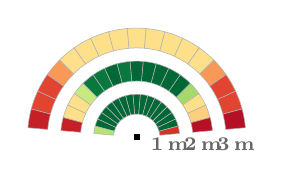
\begin{tikzpicture}[x=\fpscale cm, y=\fpscale cm, baseline=(current bounding box.north)]
  \fill[fill={rgb,1:red,0.0;green,0.408;blue,0.216}, draw=black!30, line width=0.2pt] (95.0:0.7) arc[start angle=95.0, end angle=85.0, radius=0.7] -- (85.0:1.3) arc[start angle=85.0, end angle=95.0, radius=1.3] -- cycle;
  \fill[fill={rgb,1:red,0.0;green,0.408;blue,0.216}, draw=black!30, line width=0.2pt] (105.0:0.7) arc[start angle=105.0, end angle=95.0, radius=0.7] -- (95.0:1.3) arc[start angle=95.0, end angle=105.0, radius=1.3] -- cycle;
  \fill[fill={rgb,1:red,0.0;green,0.408;blue,0.216}, draw=black!30, line width=0.2pt] (115.0:0.7) arc[start angle=115.0, end angle=105.0, radius=0.7] -- (105.0:1.3) arc[start angle=105.0, end angle=115.0, radius=1.3] -- cycle;
  \fill[fill={rgb,1:red,0.0;green,0.408;blue,0.216}, draw=black!30, line width=0.2pt] (125.0:0.7) arc[start angle=125.0, end angle=115.0, radius=0.7] -- (115.0:1.3) arc[start angle=115.0, end angle=125.0, radius=1.3] -- cycle;
  \fill[fill={rgb,1:red,0.0;green,0.408;blue,0.216}, draw=black!30, line width=0.2pt] (135.0:0.7) arc[start angle=135.0, end angle=125.0, radius=0.7] -- (125.0:1.3) arc[start angle=125.0, end angle=135.0, radius=1.3] -- cycle;
  \fill[fill={rgb,1:red,0.0;green,0.408;blue,0.216}, draw=black!30, line width=0.2pt] (145.0:0.7) arc[start angle=145.0, end angle=135.0, radius=0.7] -- (135.0:1.3) arc[start angle=135.0, end angle=145.0, radius=1.3] -- cycle;
  \fill[fill={rgb,1:red,0.0;green,0.408;blue,0.216}, draw=black!30, line width=0.2pt] (155.0:0.7) arc[start angle=155.0, end angle=145.0, radius=0.7] -- (145.0:1.3) arc[start angle=145.0, end angle=155.0, radius=1.3] -- cycle;
  \fill[fill={rgb,1:red,0.0;green,0.408;blue,0.216}, draw=black!30, line width=0.2pt] (165.0:0.7) arc[start angle=165.0, end angle=155.0, radius=0.7] -- (155.0:1.3) arc[start angle=155.0, end angle=165.0, radius=1.3] -- cycle;
  \fill[fill={rgb,1:red,0.7177;green,0.8797;blue,0.459}, draw=black!30, line width=0.2pt] (175.0:0.7) arc[start angle=175.0, end angle=165.0, radius=0.7] -- (165.0:1.3) arc[start angle=165.0, end angle=175.0, radius=1.3] -- cycle;
  \fill[fill={rgb,1:red,0.0;green,0.408;blue,0.216}, draw=black!30, line width=0.2pt] (85.0:0.7) arc[start angle=85.0, end angle=75.0, radius=0.7] -- (75.0:1.3) arc[start angle=75.0, end angle=85.0, radius=1.3] -- cycle;
  \fill[fill={rgb,1:red,0.0;green,0.408;blue,0.216}, draw=black!30, line width=0.2pt] (75.0:0.7) arc[start angle=75.0, end angle=65.0, radius=0.7] -- (65.0:1.3) arc[start angle=65.0, end angle=75.0, radius=1.3] -- cycle;
  \fill[fill={rgb,1:red,0.0;green,0.408;blue,0.216}, draw=black!30, line width=0.2pt] (65.0:0.7) arc[start angle=65.0, end angle=55.0, radius=0.7] -- (55.0:1.3) arc[start angle=55.0, end angle=65.0, radius=1.3] -- cycle;
  \fill[fill={rgb,1:red,0.0;green,0.408;blue,0.216}, draw=black!30, line width=0.2pt] (55.0:0.7) arc[start angle=55.0, end angle=45.0, radius=0.7] -- (45.0:1.3) arc[start angle=45.0, end angle=55.0, radius=1.3] -- cycle;
  \fill[fill={rgb,1:red,0.0;green,0.408;blue,0.216}, draw=black!30, line width=0.2pt] (45.0:0.7) arc[start angle=45.0, end angle=35.0, radius=0.7] -- (35.0:1.3) arc[start angle=35.0, end angle=45.0, radius=1.3] -- cycle;
  \fill[fill={rgb,1:red,0.0;green,0.408;blue,0.216}, draw=black!30, line width=0.2pt] (35.0:0.7) arc[start angle=35.0, end angle=25.0, radius=0.7] -- (25.0:1.3) arc[start angle=25.0, end angle=35.0, radius=1.3] -- cycle;
  \fill[fill={rgb,1:red,0.0;green,0.408;blue,0.216}, draw=black!30, line width=0.2pt] (25.0:0.7) arc[start angle=25.0, end angle=15.0, radius=0.7] -- (15.0:1.3) arc[start angle=15.0, end angle=25.0, radius=1.3] -- cycle;
  \fill[fill={rgb,1:red,0.843;green,0.188;blue,0.153}, draw=black!30, line width=0.2pt] (15.0:0.7) arc[start angle=15.0, end angle=5.0, radius=0.7] -- (5.0:1.3) arc[start angle=5.0, end angle=15.0, radius=1.3] -- cycle;
  \fill[fill={rgb,1:red,0.0;green,0.408;blue,0.216}, draw=black!30, line width=0.2pt] (95.0:1.7) arc[start angle=95.0, end angle=85.0, radius=1.7] -- (85.0:2.3) arc[start angle=85.0, end angle=95.0, radius=2.3] -- cycle;
  \fill[fill={rgb,1:red,0.034;green,0.4707;blue,0.2487}, draw=black!30, line width=0.2pt] (105.0:1.7) arc[start angle=105.0, end angle=95.0, radius=1.7] -- (95.0:2.3) arc[start angle=95.0, end angle=105.0, radius=2.3] -- cycle;
  \fill[fill={rgb,1:red,0.0;green,0.408;blue,0.216}, draw=black!30, line width=0.2pt] (115.0:1.7) arc[start angle=115.0, end angle=105.0, radius=1.7] -- (105.0:2.3) arc[start angle=105.0, end angle=115.0, radius=2.3] -- cycle;
  \fill[fill={rgb,1:red,0.034;green,0.4707;blue,0.2487}, draw=black!30, line width=0.2pt] (125.0:1.7) arc[start angle=125.0, end angle=115.0, radius=1.7] -- (115.0:2.3) arc[start angle=115.0, end angle=125.0, radius=2.3] -- cycle;
  \fill[fill={rgb,1:red,0.034;green,0.4707;blue,0.2487}, draw=black!30, line width=0.2pt] (135.0:1.7) arc[start angle=135.0, end angle=125.0, radius=1.7] -- (125.0:2.3) arc[start angle=125.0, end angle=135.0, radius=2.3] -- cycle;
  \fill[fill={rgb,1:red,0.7843;green,0.9083;blue,0.502}, draw=black!30, line width=0.2pt] (145.0:1.7) arc[start angle=145.0, end angle=135.0, radius=1.7] -- (135.0:2.3) arc[start angle=135.0, end angle=145.0, radius=2.3] -- cycle;
  \fill[fill={rgb,1:red,0.996;green,0.878;blue,0.545}, draw=black!30, line width=0.2pt] (155.0:1.7) arc[start angle=155.0, end angle=145.0, radius=1.7] -- (145.0:2.3) arc[start angle=145.0, end angle=155.0, radius=2.3] -- cycle;
  \fill[fill={rgb,1:red,0.996;green,0.878;blue,0.545}, draw=black!30, line width=0.2pt] (165.0:1.7) arc[start angle=165.0, end angle=155.0, radius=1.7] -- (155.0:2.3) arc[start angle=155.0, end angle=165.0, radius=2.3] -- cycle;
  \fill[fill={rgb,1:red,0.7777;green,0.1253;blue,0.1517}, draw=black!30, line width=0.2pt] (175.0:1.7) arc[start angle=175.0, end angle=165.0, radius=1.7] -- (165.0:2.3) arc[start angle=165.0, end angle=175.0, radius=2.3] -- cycle;
  \fill[fill={rgb,1:red,0.0;green,0.408;blue,0.216}, draw=black!30, line width=0.2pt] (85.0:1.7) arc[start angle=85.0, end angle=75.0, radius=1.7] -- (75.0:2.3) arc[start angle=75.0, end angle=85.0, radius=2.3] -- cycle;
  \fill[fill={rgb,1:red,0.0;green,0.408;blue,0.216}, draw=black!30, line width=0.2pt] (75.0:1.7) arc[start angle=75.0, end angle=65.0, radius=1.7] -- (65.0:2.3) arc[start angle=65.0, end angle=75.0, radius=2.3] -- cycle;
  \fill[fill={rgb,1:red,0.0;green,0.408;blue,0.216}, draw=black!30, line width=0.2pt] (65.0:1.7) arc[start angle=65.0, end angle=55.0, radius=1.7] -- (55.0:2.3) arc[start angle=55.0, end angle=65.0, radius=2.3] -- cycle;
  \fill[fill={rgb,1:red,0.0;green,0.408;blue,0.216}, draw=black!30, line width=0.2pt] (55.0:1.7) arc[start angle=55.0, end angle=45.0, radius=1.7] -- (45.0:2.3) arc[start angle=45.0, end angle=55.0, radius=2.3] -- cycle;
  \fill[fill={rgb,1:red,0.651;green,0.851;blue,0.416}, draw=black!30, line width=0.2pt] (45.0:1.7) arc[start angle=45.0, end angle=35.0, radius=1.7] -- (35.0:2.3) arc[start angle=35.0, end angle=45.0, radius=2.3] -- cycle;
  \fill[fill={rgb,1:red,0.996;green,0.878;blue,0.545}, draw=black!30, line width=0.2pt] (35.0:1.7) arc[start angle=35.0, end angle=25.0, radius=1.7] -- (25.0:2.3) arc[start angle=25.0, end angle=35.0, radius=2.3] -- cycle;
  \fill[fill={rgb,1:red,0.9947;green,0.8127;blue,0.49}, draw=black!30, line width=0.2pt] (25.0:1.7) arc[start angle=25.0, end angle=15.0, radius=1.7] -- (15.0:2.3) arc[start angle=15.0, end angle=25.0, radius=2.3] -- cycle;
  \fill[fill={rgb,1:red,0.7123;green,0.0627;blue,0.1503}, draw=black!30, line width=0.2pt] (15.0:1.7) arc[start angle=15.0, end angle=5.0, radius=1.7] -- (5.0:2.3) arc[start angle=5.0, end angle=15.0, radius=2.3] -- cycle;
  \fill[fill={rgb,1:red,0.996;green,0.878;blue,0.545}, draw=black!30, line width=0.2pt] (95.0:2.7) arc[start angle=95.0, end angle=85.0, radius=2.7] -- (85.0:3.3) arc[start angle=85.0, end angle=95.0, radius=3.3] -- cycle;
  \fill[fill={rgb,1:red,0.996;green,0.878;blue,0.545}, draw=black!30, line width=0.2pt] (105.0:2.7) arc[start angle=105.0, end angle=95.0, radius=2.7] -- (95.0:3.3) arc[start angle=95.0, end angle=105.0, radius=3.3] -- cycle;
  \fill[fill={rgb,1:red,0.996;green,0.878;blue,0.545}, draw=black!30, line width=0.2pt] (115.0:2.7) arc[start angle=115.0, end angle=105.0, radius=2.7] -- (105.0:3.3) arc[start angle=105.0, end angle=115.0, radius=3.3] -- cycle;
  \fill[fill={rgb,1:red,0.996;green,0.878;blue,0.545}, draw=black!30, line width=0.2pt] (125.0:2.7) arc[start angle=125.0, end angle=115.0, radius=2.7] -- (115.0:3.3) arc[start angle=115.0, end angle=125.0, radius=3.3] -- cycle;
  \fill[fill={rgb,1:red,0.996;green,0.878;blue,0.545}, draw=black!30, line width=0.2pt] (135.0:2.7) arc[start angle=135.0, end angle=125.0, radius=2.7] -- (125.0:3.3) arc[start angle=125.0, end angle=135.0, radius=3.3] -- cycle;
  \fill[fill={rgb,1:red,0.9803;green,0.597;blue,0.341}, draw=black!30, line width=0.2pt] (145.0:2.7) arc[start angle=145.0, end angle=135.0, radius=2.7] -- (135.0:3.3) arc[start angle=135.0, end angle=145.0, radius=3.3] -- cycle;
  \fill[fill={rgb,1:red,0.881;green,0.2677;blue,0.1897}, draw=black!30, line width=0.2pt] (155.0:2.7) arc[start angle=155.0, end angle=145.0, radius=2.7] -- (145.0:3.3) arc[start angle=145.0, end angle=155.0, radius=3.3] -- cycle;
  \fill[fill={rgb,1:red,0.881;green,0.2677;blue,0.1897}, draw=black!30, line width=0.2pt] (165.0:2.7) arc[start angle=165.0, end angle=155.0, radius=2.7] -- (155.0:3.3) arc[start angle=155.0, end angle=165.0, radius=3.3] -- cycle;
  \fill[fill={rgb,1:red,0.7777;green,0.1253;blue,0.1517}, draw=black!30, line width=0.2pt] (175.0:2.7) arc[start angle=175.0, end angle=165.0, radius=2.7] -- (165.0:3.3) arc[start angle=165.0, end angle=175.0, radius=3.3] -- cycle;
  \fill[fill={rgb,1:red,0.996;green,0.878;blue,0.545}, draw=black!30, line width=0.2pt] (85.0:2.7) arc[start angle=85.0, end angle=75.0, radius=2.7] -- (75.0:3.3) arc[start angle=75.0, end angle=85.0, radius=3.3] -- cycle;
  \fill[fill={rgb,1:red,0.996;green,0.878;blue,0.545}, draw=black!30, line width=0.2pt] (75.0:2.7) arc[start angle=75.0, end angle=65.0, radius=2.7] -- (65.0:3.3) arc[start angle=65.0, end angle=75.0, radius=3.3] -- cycle;
  \fill[fill={rgb,1:red,0.996;green,0.878;blue,0.545}, draw=black!30, line width=0.2pt] (65.0:2.7) arc[start angle=65.0, end angle=55.0, radius=2.7] -- (55.0:3.3) arc[start angle=55.0, end angle=65.0, radius=3.3] -- cycle;
  \fill[fill={rgb,1:red,0.996;green,0.878;blue,0.545}, draw=black!30, line width=0.2pt] (55.0:2.7) arc[start angle=55.0, end angle=45.0, radius=2.7] -- (45.0:3.3) arc[start angle=45.0, end angle=55.0, radius=3.3] -- cycle;
  \fill[fill={rgb,1:red,0.9803;green,0.597;blue,0.341}, draw=black!30, line width=0.2pt] (45.0:2.7) arc[start angle=45.0, end angle=35.0, radius=2.7] -- (35.0:3.3) arc[start angle=35.0, end angle=45.0, radius=3.3] -- cycle;
  \fill[fill={rgb,1:red,0.881;green,0.2677;blue,0.1897}, draw=black!30, line width=0.2pt] (35.0:2.7) arc[start angle=35.0, end angle=25.0, radius=2.7] -- (25.0:3.3) arc[start angle=25.0, end angle=35.0, radius=3.3] -- cycle;
  \fill[fill={rgb,1:red,0.881;green,0.2677;blue,0.1897}, draw=black!30, line width=0.2pt] (25.0:2.7) arc[start angle=25.0, end angle=15.0, radius=2.7] -- (15.0:3.3) arc[start angle=15.0, end angle=25.0, radius=3.3] -- cycle;
  \fill[fill={rgb,1:red,0.7123;green,0.0627;blue,0.1503}, draw=black!30, line width=0.2pt] (15.0:2.7) arc[start angle=15.0, end angle=5.0, radius=2.7] -- (5.0:3.3) arc[start angle=5.0, end angle=15.0, radius=3.3] -- cycle;
  \fill[black] (-0.09, -0.09) rectangle (0.09, 0.09);
  \node[font=\scriptsize\bfseries, text=black!60] at (1, -0.22) {1\,m};
  \node[font=\scriptsize\bfseries, text=black!60] at (2, -0.22) {2\,m};
  \node[font=\scriptsize\bfseries, text=black!60] at (3, -0.22) {3\,m};
\end{tikzpicture}
 & % floorplan colorbar: det — generated, edit freely
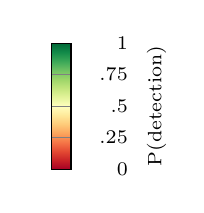
\begin{tikzpicture}[baseline=(current bounding box.north)]
\pgfplotsset{colormap={rdylgnrev}{rgb=(0.0,0.408,0.216) rgb=(0.0729,0.5423,0.286) rgb=(0.2297,0.6581,0.3457) rgb=(0.4359,0.7567,0.392) rgb=(0.6151,0.8353,0.412) rgb=(0.7653,0.9001,0.4897) rgb=(0.8936,0.955,0.6033) rgb=(1.0,1.0,0.749) rgb=(0.9971,0.9129,0.6033) rgb=(0.9943,0.794,0.4743) rgb=(0.987,0.6456,0.3633) rgb=(0.962,0.4634,0.2797) rgb=(0.8919,0.2904,0.2001) rgb=(0.787,0.1343,0.1519) rgb=(0.647,0.0,0.149)}, colormap={rdylgn}{rgb=(0.647,0.0,0.149) rgb=(0.787,0.1343,0.1519) rgb=(0.8919,0.2904,0.2001) rgb=(0.962,0.4634,0.2797) rgb=(0.987,0.6456,0.3633) rgb=(0.9943,0.794,0.4743) rgb=(0.9971,0.9129,0.6033) rgb=(1.0,1.0,0.749) rgb=(0.8936,0.955,0.6033) rgb=(0.7653,0.9001,0.4897) rgb=(0.6151,0.8353,0.412) rgb=(0.4359,0.7567,0.392) rgb=(0.2297,0.6581,0.3457) rgb=(0.0729,0.5423,0.286) rgb=(0.0,0.408,0.216)}}
\begin{axis}[hide axis, scale only axis, width=0pt, height=1.6cm,
  colormap name=rdylgn, colorbar, point meta min=0.0, point meta max=1.0,
  colorbar style={height=1.6cm, width=0.25cm, ylabel={P(detection)}, ylabel style={font=\scriptsize},
    ytick={0.0,0.25,0.5,0.75,1.0}, yticklabels={0,.25,.5,.75,1}, tick label style={font=\scriptsize},
    yticklabel style={text width=1.7em, align=right}}]
  \addplot[draw=none] coordinates {(0,0)};
\end{axis}
\end{tikzpicture}
 \\[2pt]
\multicolumn{3}{c}{(a) Probability of Detection} & \\[8pt]
% floorplan fan: BlobBoards / trans — generated, edit freely
\providecommand{\fpscale}{1}
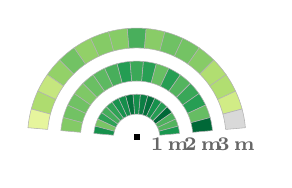
\begin{tikzpicture}[x=\fpscale cm, y=\fpscale cm, baseline=(current bounding box.north)]
  \fill[fill={rgb,1:red,0.081;green,0.5573;blue,0.2938}, draw=black!30, line width=0.2pt] (95.0:0.7) arc[start angle=95.0, end angle=85.0, radius=0.7] -- (85.0:1.3) arc[start angle=85.0, end angle=95.0, radius=1.3] -- cycle;
  \fill[fill={rgb,1:red,0.0204;green,0.4457;blue,0.2356}, draw=black!30, line width=0.2pt] (105.0:0.7) arc[start angle=105.0, end angle=95.0, radius=0.7] -- (95.0:1.3) arc[start angle=95.0, end angle=105.0, radius=1.3] -- cycle;
  \fill[fill={rgb,1:red,0.081;green,0.5573;blue,0.2938}, draw=black!30, line width=0.2pt] (115.0:0.7) arc[start angle=115.0, end angle=105.0, radius=0.7] -- (105.0:1.3) arc[start angle=105.0, end angle=115.0, radius=1.3] -- cycle;
  \fill[fill={rgb,1:red,0.0901;green,0.574;blue,0.3025}, draw=black!30, line width=0.2pt] (125.0:0.7) arc[start angle=125.0, end angle=115.0, radius=0.7] -- (115.0:1.3) arc[start angle=115.0, end angle=125.0, radius=1.3] -- cycle;
  \fill[fill={rgb,1:red,0.1854;green,0.6366;blue,0.3347}, draw=black!30, line width=0.2pt] (135.0:0.7) arc[start angle=135.0, end angle=125.0, radius=0.7] -- (125.0:1.3) arc[start angle=125.0, end angle=135.0, radius=1.3] -- cycle;
  \fill[fill={rgb,1:red,0.2705;green,0.678;blue,0.3558}, draw=black!30, line width=0.2pt] (145.0:0.7) arc[start angle=145.0, end angle=135.0, radius=0.7] -- (135.0:1.3) arc[start angle=135.0, end angle=145.0, radius=1.3] -- cycle;
  \fill[fill={rgb,1:red,0.1747;green,0.6314;blue,0.332}, draw=black!30, line width=0.2pt] (155.0:0.7) arc[start angle=155.0, end angle=145.0, radius=0.7] -- (145.0:1.3) arc[start angle=145.0, end angle=155.0, radius=1.3] -- cycle;
  \fill[fill={rgb,1:red,0.4732;green,0.7731;blue,0.3962}, draw=black!30, line width=0.2pt] (165.0:0.7) arc[start angle=165.0, end angle=155.0, radius=0.7] -- (155.0:1.3) arc[start angle=155.0, end angle=165.0, radius=1.3] -- cycle;
  \fill[fill={rgb,1:red,0.0873;green,0.569;blue,0.2999}, draw=black!30, line width=0.2pt] (175.0:0.7) arc[start angle=175.0, end angle=165.0, radius=0.7] -- (165.0:1.3) arc[start angle=165.0, end angle=175.0, radius=1.3] -- cycle;
  \fill[fill={rgb,1:red,0.047;green,0.4946;blue,0.2611}, draw=black!30, line width=0.2pt] (85.0:0.7) arc[start angle=85.0, end angle=75.0, radius=0.7] -- (75.0:1.3) arc[start angle=75.0, end angle=85.0, radius=1.3] -- cycle;
  \fill[fill={rgb,1:red,0.0171;green,0.4395;blue,0.2324}, draw=black!30, line width=0.2pt] (75.0:0.7) arc[start angle=75.0, end angle=65.0, radius=0.7] -- (65.0:1.3) arc[start angle=65.0, end angle=75.0, radius=1.3] -- cycle;
  \fill[fill={rgb,1:red,0.0864;green,0.5673;blue,0.299}, draw=black!30, line width=0.2pt] (65.0:0.7) arc[start angle=65.0, end angle=55.0, radius=0.7] -- (55.0:1.3) arc[start angle=55.0, end angle=65.0, radius=1.3] -- cycle;
  \fill[fill={rgb,1:red,0.1382;green,0.6136;blue,0.323}, draw=black!30, line width=0.2pt] (55.0:0.7) arc[start angle=55.0, end angle=45.0, radius=0.7] -- (45.0:1.3) arc[start angle=45.0, end angle=55.0, radius=1.3] -- cycle;
  \fill[fill={rgb,1:red,0.0;green,0.408;blue,0.216}, draw=black!30, line width=0.2pt] (45.0:0.7) arc[start angle=45.0, end angle=35.0, radius=0.7] -- (35.0:1.3) arc[start angle=35.0, end angle=45.0, radius=1.3] -- cycle;
  \fill[fill={rgb,1:red,0.3006;green,0.6926;blue,0.3633}, draw=black!30, line width=0.2pt] (35.0:0.7) arc[start angle=35.0, end angle=25.0, radius=0.7] -- (25.0:1.3) arc[start angle=25.0, end angle=35.0, radius=1.3] -- cycle;
  \fill[fill={rgb,1:red,0.326;green,0.705;blue,0.3696}, draw=black!30, line width=0.2pt] (25.0:0.7) arc[start angle=25.0, end angle=15.0, radius=0.7] -- (15.0:1.3) arc[start angle=15.0, end angle=25.0, radius=1.3] -- cycle;
  \fill[fill={rgb,1:red,0.0993;green,0.591;blue,0.3114}, draw=black!30, line width=0.2pt] (15.0:0.7) arc[start angle=15.0, end angle=5.0, radius=0.7] -- (5.0:1.3) arc[start angle=5.0, end angle=15.0, radius=1.3] -- cycle;
  \fill[fill={rgb,1:red,0.142;green,0.6155;blue,0.3239}, draw=black!30, line width=0.2pt] (105.0:1.7) arc[start angle=105.0, end angle=95.0, radius=1.7] -- (95.0:2.3) arc[start angle=95.0, end angle=105.0, radius=2.3] -- cycle;
  \fill[fill={rgb,1:red,0.1577;green,0.6231;blue,0.3278}, draw=black!30, line width=0.2pt] (85.0:1.7) arc[start angle=85.0, end angle=75.0, radius=1.7] -- (75.0:2.3) arc[start angle=75.0, end angle=85.0, radius=2.3] -- cycle;
  \fill[fill={rgb,1:red,0.2815;green,0.6834;blue,0.3586}, draw=black!30, line width=0.2pt] (115.0:1.7) arc[start angle=115.0, end angle=105.0, radius=1.7] -- (105.0:2.3) arc[start angle=105.0, end angle=115.0, radius=2.3] -- cycle;
  \fill[fill={rgb,1:red,0.3666;green,0.7248;blue,0.3797}, draw=black!30, line width=0.2pt] (125.0:1.7) arc[start angle=125.0, end angle=115.0, radius=1.7] -- (115.0:2.3) arc[start angle=115.0, end angle=125.0, radius=2.3] -- cycle;
  \fill[fill={rgb,1:red,0.4169;green,0.7484;blue,0.3899}, draw=black!30, line width=0.2pt] (135.0:1.7) arc[start angle=135.0, end angle=125.0, radius=1.7] -- (125.0:2.3) arc[start angle=125.0, end angle=135.0, radius=2.3] -- cycle;
  \fill[fill={rgb,1:red,0.4979;green,0.7839;blue,0.3989}, draw=black!30, line width=0.2pt] (145.0:1.7) arc[start angle=145.0, end angle=135.0, radius=1.7] -- (135.0:2.3) arc[start angle=135.0, end angle=145.0, radius=2.3] -- cycle;
  \fill[fill={rgb,1:red,0.4378;green,0.7576;blue,0.3922}, draw=black!30, line width=0.2pt] (155.0:1.7) arc[start angle=155.0, end angle=145.0, radius=1.7] -- (145.0:2.3) arc[start angle=145.0, end angle=155.0, radius=2.3] -- cycle;
  \fill[fill={rgb,1:red,0.446;green,0.7612;blue,0.3931}, draw=black!30, line width=0.2pt] (165.0:1.7) arc[start angle=165.0, end angle=155.0, radius=1.7] -- (155.0:2.3) arc[start angle=155.0, end angle=165.0, radius=2.3] -- cycle;
  \fill[fill={rgb,1:red,0.5128;green,0.7904;blue,0.4006}, draw=black!30, line width=0.2pt] (175.0:1.7) arc[start angle=175.0, end angle=165.0, radius=1.7] -- (165.0:2.3) arc[start angle=165.0, end angle=175.0, radius=2.3] -- cycle;
  \fill[fill={rgb,1:red,0.2317;green,0.6591;blue,0.3462}, draw=black!30, line width=0.2pt] (95.0:1.7) arc[start angle=95.0, end angle=85.0, radius=1.7] -- (85.0:2.3) arc[start angle=85.0, end angle=95.0, radius=2.3] -- cycle;
  \fill[fill={rgb,1:red,0.4072;green,0.7442;blue,0.3888}, draw=black!30, line width=0.2pt] (75.0:1.7) arc[start angle=75.0, end angle=65.0, radius=1.7] -- (65.0:2.3) arc[start angle=65.0, end angle=75.0, radius=2.3] -- cycle;
  \fill[fill={rgb,1:red,0.1483;green,0.6185;blue,0.3255}, draw=black!30, line width=0.2pt] (65.0:1.7) arc[start angle=65.0, end angle=55.0, radius=1.7] -- (55.0:2.3) arc[start angle=55.0, end angle=65.0, radius=2.3] -- cycle;
  \fill[fill={rgb,1:red,0.3262;green,0.7051;blue,0.3697}, draw=black!30, line width=0.2pt] (55.0:1.7) arc[start angle=55.0, end angle=45.0, radius=1.7] -- (45.0:2.3) arc[start angle=45.0, end angle=55.0, radius=2.3] -- cycle;
  \fill[fill={rgb,1:red,0.225;green,0.6558;blue,0.3445}, draw=black!30, line width=0.2pt] (45.0:1.7) arc[start angle=45.0, end angle=35.0, radius=1.7] -- (35.0:2.3) arc[start angle=35.0, end angle=45.0, radius=2.3] -- cycle;
  \fill[fill={rgb,1:red,0.149;green,0.6189;blue,0.3257}, draw=black!30, line width=0.2pt] (35.0:1.7) arc[start angle=35.0, end angle=25.0, radius=1.7] -- (25.0:2.3) arc[start angle=25.0, end angle=35.0, radius=2.3] -- cycle;
  \fill[fill={rgb,1:red,0.3983;green,0.7402;blue,0.3876}, draw=black!30, line width=0.2pt] (25.0:1.7) arc[start angle=25.0, end angle=15.0, radius=1.7] -- (15.0:2.3) arc[start angle=15.0, end angle=25.0, radius=2.3] -- cycle;
  \fill[fill={rgb,1:red,0.0;green,0.408;blue,0.216}, draw=black!30, line width=0.2pt] (15.0:1.7) arc[start angle=15.0, end angle=5.0, radius=1.7] -- (5.0:2.3) arc[start angle=5.0, end angle=15.0, radius=2.3] -- cycle;
  \fill[fill={rgb,1:red,0.2857;green,0.6854;blue,0.3596}, draw=black!30, line width=0.2pt] (95.0:2.7) arc[start angle=95.0, end angle=85.0, radius=2.7] -- (85.0:3.3) arc[start angle=85.0, end angle=95.0, radius=3.3] -- cycle;
  \fill[fill={rgb,1:red,0.5308;green,0.7983;blue,0.4026}, draw=black!30, line width=0.2pt] (105.0:2.7) arc[start angle=105.0, end angle=95.0, radius=2.7] -- (95.0:3.3) arc[start angle=95.0, end angle=105.0, radius=3.3] -- cycle;
  \fill[fill={rgb,1:red,0.5228;green,0.7948;blue,0.4017}, draw=black!30, line width=0.2pt] (115.0:2.7) arc[start angle=115.0, end angle=105.0, radius=2.7] -- (105.0:3.3) arc[start angle=105.0, end angle=115.0, radius=3.3] -- cycle;
  \fill[fill={rgb,1:red,0.5737;green,0.8171;blue,0.4074}, draw=black!30, line width=0.2pt] (125.0:2.7) arc[start angle=125.0, end angle=115.0, radius=2.7] -- (115.0:3.3) arc[start angle=115.0, end angle=125.0, radius=3.3] -- cycle;
  \fill[fill={rgb,1:red,0.4472;green,0.7617;blue,0.3933}, draw=black!30, line width=0.2pt] (135.0:2.7) arc[start angle=135.0, end angle=125.0, radius=2.7] -- (125.0:3.3) arc[start angle=125.0, end angle=135.0, radius=3.3] -- cycle;
  \fill[fill={rgb,1:red,0.5783;green,0.8191;blue,0.4079}, draw=black!30, line width=0.2pt] (145.0:2.7) arc[start angle=145.0, end angle=135.0, radius=2.7] -- (135.0:3.3) arc[start angle=135.0, end angle=145.0, radius=3.3] -- cycle;
  \fill[fill={rgb,1:red,0.7715;green,0.9028;blue,0.4937}, draw=black!30, line width=0.2pt] (155.0:2.7) arc[start angle=155.0, end angle=145.0, radius=2.7] -- (145.0:3.3) arc[start angle=145.0, end angle=155.0, radius=3.3] -- cycle;
  \fill[fill={rgb,1:red,0.6817;green,0.8642;blue,0.4358}, draw=black!30, line width=0.2pt] (165.0:2.7) arc[start angle=165.0, end angle=155.0, radius=2.7] -- (155.0:3.3) arc[start angle=155.0, end angle=165.0, radius=3.3] -- cycle;
  \fill[fill={rgb,1:red,0.9038;green,0.9593;blue,0.6173}, draw=black!30, line width=0.2pt] (175.0:2.7) arc[start angle=175.0, end angle=165.0, radius=2.7] -- (165.0:3.3) arc[start angle=165.0, end angle=175.0, radius=3.3] -- cycle;
  \fill[fill={rgb,1:red,0.538;green,0.8015;blue,0.4034}, draw=black!30, line width=0.2pt] (85.0:2.7) arc[start angle=85.0, end angle=75.0, radius=2.7] -- (75.0:3.3) arc[start angle=75.0, end angle=85.0, radius=3.3] -- cycle;
  \fill[fill={rgb,1:red,0.435;green,0.7563;blue,0.3919}, draw=black!30, line width=0.2pt] (75.0:2.7) arc[start angle=75.0, end angle=65.0, radius=2.7] -- (65.0:3.3) arc[start angle=65.0, end angle=75.0, radius=3.3] -- cycle;
  \fill[fill={rgb,1:red,0.4536;green,0.7645;blue,0.394}, draw=black!30, line width=0.2pt] (65.0:2.7) arc[start angle=65.0, end angle=55.0, radius=2.7] -- (55.0:3.3) arc[start angle=55.0, end angle=65.0, radius=3.3] -- cycle;
  \fill[fill={rgb,1:red,0.529;green,0.7975;blue,0.4024}, draw=black!30, line width=0.2pt] (55.0:2.7) arc[start angle=55.0, end angle=45.0, radius=2.7] -- (45.0:3.3) arc[start angle=45.0, end angle=55.0, radius=3.3] -- cycle;
  \fill[fill={rgb,1:red,0.694;green,0.8695;blue,0.4438}, draw=black!30, line width=0.2pt] (45.0:2.7) arc[start angle=45.0, end angle=35.0, radius=2.7] -- (35.0:3.3) arc[start angle=35.0, end angle=45.0, radius=3.3] -- cycle;
  \fill[fill={rgb,1:red,0.6926;green,0.8689;blue,0.4428}, draw=black!30, line width=0.2pt] (35.0:2.7) arc[start angle=35.0, end angle=25.0, radius=2.7] -- (25.0:3.3) arc[start angle=25.0, end angle=35.0, radius=3.3] -- cycle;
  \fill[fill={rgb,1:red,0.8204;green,0.9239;blue,0.5253}, draw=black!30, line width=0.2pt] (25.0:2.7) arc[start angle=25.0, end angle=15.0, radius=2.7] -- (15.0:3.3) arc[start angle=15.0, end angle=25.0, radius=3.3] -- cycle;
  \fill[fill=gray!30, draw=black!30, line width=0.2pt] (15.0:2.7) arc[start angle=15.0, end angle=5.0, radius=2.7] -- (5.0:3.3) arc[start angle=5.0, end angle=15.0, radius=3.3] -- cycle;
  \fill[black] (-0.09, -0.09) rectangle (0.09, 0.09);
  \node[font=\scriptsize\bfseries, text=black!60] at (1, -0.22) {1\,m};
  \node[font=\scriptsize\bfseries, text=black!60] at (2, -0.22) {2\,m};
  \node[font=\scriptsize\bfseries, text=black!60] at (3, -0.22) {3\,m};
\end{tikzpicture}
 & % floorplan fan: AprilTag / trans — generated, edit freely
\providecommand{\fpscale}{1}
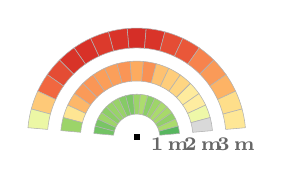
\begin{tikzpicture}[x=\fpscale cm, y=\fpscale cm, baseline=(current bounding box.north)]
  \fill[fill={rgb,1:red,0.6113;green,0.8336;blue,0.4116}, draw=black!30, line width=0.2pt] (95.0:0.7) arc[start angle=95.0, end angle=85.0, radius=0.7] -- (85.0:1.3) arc[start angle=85.0, end angle=95.0, radius=1.3] -- cycle;
  \fill[fill={rgb,1:red,0.493;green,0.7818;blue,0.3984}, draw=black!30, line width=0.2pt] (105.0:0.7) arc[start angle=105.0, end angle=95.0, radius=0.7] -- (95.0:1.3) arc[start angle=95.0, end angle=105.0, radius=1.3] -- cycle;
  \fill[fill={rgb,1:red,0.5242;green,0.7955;blue,0.4019}, draw=black!30, line width=0.2pt] (115.0:0.7) arc[start angle=115.0, end angle=105.0, radius=0.7] -- (105.0:1.3) arc[start angle=105.0, end angle=115.0, radius=1.3] -- cycle;
  \fill[fill={rgb,1:red,0.5997;green,0.8285;blue,0.4103}, draw=black!30, line width=0.2pt] (125.0:0.7) arc[start angle=125.0, end angle=115.0, radius=0.7] -- (115.0:1.3) arc[start angle=115.0, end angle=125.0, radius=1.3] -- cycle;
  \fill[fill={rgb,1:red,0.5965;green,0.8271;blue,0.4099}, draw=black!30, line width=0.2pt] (135.0:0.7) arc[start angle=135.0, end angle=125.0, radius=0.7] -- (125.0:1.3) arc[start angle=125.0, end angle=135.0, radius=1.3] -- cycle;
  \fill[fill={rgb,1:red,0.5517;green,0.8075;blue,0.4049}, draw=black!30, line width=0.2pt] (145.0:0.7) arc[start angle=145.0, end angle=135.0, radius=0.7] -- (135.0:1.3) arc[start angle=135.0, end angle=145.0, radius=1.3] -- cycle;
  \fill[fill={rgb,1:red,0.6177;green,0.8364;blue,0.4123}, draw=black!30, line width=0.2pt] (155.0:0.7) arc[start angle=155.0, end angle=145.0, radius=0.7] -- (145.0:1.3) arc[start angle=145.0, end angle=155.0, radius=1.3] -- cycle;
  \fill[fill={rgb,1:red,0.4755;green,0.7741;blue,0.3964}, draw=black!30, line width=0.2pt] (165.0:0.7) arc[start angle=165.0, end angle=155.0, radius=0.7] -- (155.0:1.3) arc[start angle=155.0, end angle=165.0, radius=1.3] -- cycle;
  \fill[fill={rgb,1:red,0.4512;green,0.7634;blue,0.3937}, draw=black!30, line width=0.2pt] (175.0:0.7) arc[start angle=175.0, end angle=165.0, radius=0.7] -- (165.0:1.3) arc[start angle=165.0, end angle=175.0, radius=1.3] -- cycle;
  \fill[fill={rgb,1:red,0.6742;green,0.861;blue,0.431}, draw=black!30, line width=0.2pt] (85.0:0.7) arc[start angle=85.0, end angle=75.0, radius=0.7] -- (75.0:1.3) arc[start angle=75.0, end angle=85.0, radius=1.3] -- cycle;
  \fill[fill={rgb,1:red,0.5483;green,0.806;blue,0.4045}, draw=black!30, line width=0.2pt] (75.0:0.7) arc[start angle=75.0, end angle=65.0, radius=0.7] -- (65.0:1.3) arc[start angle=65.0, end angle=75.0, radius=1.3] -- cycle;
  \fill[fill={rgb,1:red,0.6192;green,0.8371;blue,0.4125}, draw=black!30, line width=0.2pt] (65.0:0.7) arc[start angle=65.0, end angle=55.0, radius=0.7] -- (55.0:1.3) arc[start angle=55.0, end angle=65.0, radius=1.3] -- cycle;
  \fill[fill={rgb,1:red,0.6655;green,0.8572;blue,0.4253}, draw=black!30, line width=0.2pt] (55.0:0.7) arc[start angle=55.0, end angle=45.0, radius=0.7] -- (45.0:1.3) arc[start angle=45.0, end angle=55.0, radius=1.3] -- cycle;
  \fill[fill={rgb,1:red,0.6533;green,0.852;blue,0.4175}, draw=black!30, line width=0.2pt] (45.0:0.7) arc[start angle=45.0, end angle=35.0, radius=0.7] -- (35.0:1.3) arc[start angle=35.0, end angle=45.0, radius=1.3] -- cycle;
  \fill[fill={rgb,1:red,0.5745;green,0.8175;blue,0.4075}, draw=black!30, line width=0.2pt] (35.0:0.7) arc[start angle=35.0, end angle=25.0, radius=0.7] -- (25.0:1.3) arc[start angle=25.0, end angle=35.0, radius=1.3] -- cycle;
  \fill[fill={rgb,1:red,0.6683;green,0.8584;blue,0.4271}, draw=black!30, line width=0.2pt] (25.0:0.7) arc[start angle=25.0, end angle=15.0, radius=0.7] -- (15.0:1.3) arc[start angle=15.0, end angle=25.0, radius=1.3] -- cycle;
  \fill[fill={rgb,1:red,0.3423;green,0.7129;blue,0.3737}, draw=black!30, line width=0.2pt] (15.0:0.7) arc[start angle=15.0, end angle=5.0, radius=0.7] -- (5.0:1.3) arc[start angle=5.0, end angle=15.0, radius=1.3] -- cycle;
  \fill[fill={rgb,1:red,0.9842;green,0.6251;blue,0.3539}, draw=black!30, line width=0.2pt] (115.0:1.7) arc[start angle=115.0, end angle=105.0, radius=1.7] -- (105.0:2.3) arc[start angle=105.0, end angle=115.0, radius=2.3] -- cycle;
  \fill[fill={rgb,1:red,0.9787;green,0.5851;blue,0.3355}, draw=black!30, line width=0.2pt] (105.0:1.7) arc[start angle=105.0, end angle=95.0, radius=1.7] -- (95.0:2.3) arc[start angle=95.0, end angle=105.0, radius=2.3] -- cycle;
  \fill[fill={rgb,1:red,0.9767;green,0.5703;blue,0.3287}, draw=black!30, line width=0.2pt] (85.0:1.7) arc[start angle=85.0, end angle=75.0, radius=1.7] -- (75.0:2.3) arc[start angle=75.0, end angle=85.0, radius=2.3] -- cycle;
  \fill[fill={rgb,1:red,0.9832;green,0.6181;blue,0.3507}, draw=black!30, line width=0.2pt] (125.0:1.7) arc[start angle=125.0, end angle=115.0, radius=1.7] -- (115.0:2.3) arc[start angle=115.0, end angle=125.0, radius=2.3] -- cycle;
  \fill[fill={rgb,1:red,0.9792;green,0.589;blue,0.3373}, draw=black!30, line width=0.2pt] (135.0:1.7) arc[start angle=135.0, end angle=125.0, radius=1.7] -- (125.0:2.3) arc[start angle=125.0, end angle=135.0, radius=2.3] -- cycle;
  \fill[fill={rgb,1:red,0.9814;green,0.6045;blue,0.3445}, draw=black!30, line width=0.2pt] (145.0:1.7) arc[start angle=145.0, end angle=135.0, radius=1.7] -- (135.0:2.3) arc[start angle=135.0, end angle=145.0, radius=2.3] -- cycle;
  \fill[fill={rgb,1:red,0.9928;green,0.719;blue,0.4111}, draw=black!30, line width=0.2pt] (155.0:1.7) arc[start angle=155.0, end angle=145.0, radius=1.7] -- (145.0:2.3) arc[start angle=145.0, end angle=155.0, radius=2.3] -- cycle;
  \fill[fill={rgb,1:red,0.9966;green,0.8973;blue,0.5773}, draw=black!30, line width=0.2pt] (165.0:1.7) arc[start angle=165.0, end angle=155.0, radius=1.7] -- (155.0:2.3) arc[start angle=155.0, end angle=165.0, radius=2.3] -- cycle;
  \fill[fill={rgb,1:red,0.6106;green,0.8333;blue,0.4115}, draw=black!30, line width=0.2pt] (175.0:1.7) arc[start angle=175.0, end angle=165.0, radius=1.7] -- (165.0:2.3) arc[start angle=165.0, end angle=175.0, radius=2.3] -- cycle;
  \fill[fill={rgb,1:red,0.9903;green,0.6693;blue,0.3742}, draw=black!30, line width=0.2pt] (95.0:1.7) arc[start angle=95.0, end angle=85.0, radius=1.7] -- (85.0:2.3) arc[start angle=85.0, end angle=95.0, radius=2.3] -- cycle;
  \fill[fill={rgb,1:red,0.9936;green,0.7583;blue,0.4442}, draw=black!30, line width=0.2pt] (75.0:1.7) arc[start angle=75.0, end angle=65.0, radius=1.7] -- (65.0:2.3) arc[start angle=65.0, end angle=75.0, radius=2.3] -- cycle;
  \fill[fill={rgb,1:red,0.9945;green,0.8033;blue,0.4821}, draw=black!30, line width=0.2pt] (65.0:1.7) arc[start angle=65.0, end angle=55.0, radius=1.7] -- (55.0:2.3) arc[start angle=55.0, end angle=65.0, radius=2.3] -- cycle;
  \fill[fill={rgb,1:red,0.9951;green,0.8353;blue,0.5091}, draw=black!30, line width=0.2pt] (55.0:1.7) arc[start angle=55.0, end angle=45.0, radius=1.7] -- (45.0:2.3) arc[start angle=45.0, end angle=55.0, radius=2.3] -- cycle;
  \fill[fill={rgb,1:red,0.9974;green,0.9209;blue,0.6167}, draw=black!30, line width=0.2pt] (45.0:1.7) arc[start angle=45.0, end angle=35.0, radius=1.7] -- (35.0:2.3) arc[start angle=35.0, end angle=45.0, radius=2.3] -- cycle;
  \fill[fill={rgb,1:red,0.9976;green,0.9265;blue,0.626}, draw=black!30, line width=0.2pt] (35.0:1.7) arc[start angle=35.0, end angle=25.0, radius=1.7] -- (25.0:2.3) arc[start angle=25.0, end angle=35.0, radius=2.3] -- cycle;
  \fill[fill={rgb,1:red,0.9341;green,0.9721;blue,0.6587}, draw=black!30, line width=0.2pt] (25.0:1.7) arc[start angle=25.0, end angle=15.0, radius=1.7] -- (15.0:2.3) arc[start angle=15.0, end angle=25.0, radius=2.3] -- cycle;
  \fill[fill=gray!30, draw=black!30, line width=0.2pt] (15.0:1.7) arc[start angle=15.0, end angle=5.0, radius=1.7] -- (5.0:2.3) arc[start angle=5.0, end angle=15.0, radius=2.3] -- cycle;
  \fill[fill={rgb,1:red,0.837;green,0.1823;blue,0.1529}, draw=black!30, line width=0.2pt] (95.0:2.7) arc[start angle=95.0, end angle=85.0, radius=2.7] -- (85.0:3.3) arc[start angle=85.0, end angle=95.0, radius=3.3] -- cycle;
  \fill[fill={rgb,1:red,0.85;green,0.2026;blue,0.1597}, draw=black!30, line width=0.2pt] (105.0:2.7) arc[start angle=105.0, end angle=95.0, radius=2.7] -- (95.0:3.3) arc[start angle=95.0, end angle=105.0, radius=3.3] -- cycle;
  \fill[fill={rgb,1:red,0.8626;green,0.229;blue,0.1719}, draw=black!30, line width=0.2pt] (115.0:2.7) arc[start angle=115.0, end angle=105.0, radius=2.7] -- (105.0:3.3) arc[start angle=105.0, end angle=115.0, radius=3.3] -- cycle;
  \fill[fill={rgb,1:red,0.8454;green,0.1931;blue,0.1553}, draw=black!30, line width=0.2pt] (125.0:2.7) arc[start angle=125.0, end angle=115.0, radius=2.7] -- (115.0:3.3) arc[start angle=115.0, end angle=125.0, radius=3.3] -- cycle;
  \fill[fill={rgb,1:red,0.8485;green,0.1996;blue,0.1583}, draw=black!30, line width=0.2pt] (135.0:2.7) arc[start angle=135.0, end angle=125.0, radius=2.7] -- (125.0:3.3) arc[start angle=125.0, end angle=135.0, radius=3.3] -- cycle;
  \fill[fill={rgb,1:red,0.8953;green,0.2977;blue,0.2035}, draw=black!30, line width=0.2pt] (145.0:2.7) arc[start angle=145.0, end angle=135.0, radius=2.7] -- (135.0:3.3) arc[start angle=135.0, end angle=145.0, radius=3.3] -- cycle;
  \fill[fill={rgb,1:red,0.946;green,0.404;blue,0.2524}, draw=black!30, line width=0.2pt] (155.0:2.7) arc[start angle=155.0, end angle=145.0, radius=2.7] -- (145.0:3.3) arc[start angle=145.0, end angle=155.0, radius=3.3] -- cycle;
  \fill[fill={rgb,1:red,0.9942;green,0.7879;blue,0.4692}, draw=black!30, line width=0.2pt] (165.0:2.7) arc[start angle=165.0, end angle=155.0, radius=2.7] -- (155.0:3.3) arc[start angle=155.0, end angle=165.0, radius=3.3] -- cycle;
  \fill[fill={rgb,1:red,0.9262;green,0.9688;blue,0.6479}, draw=black!30, line width=0.2pt] (175.0:2.7) arc[start angle=175.0, end angle=165.0, radius=2.7] -- (165.0:3.3) arc[start angle=165.0, end angle=175.0, radius=3.3] -- cycle;
  \fill[fill={rgb,1:red,0.8505;green,0.2037;blue,0.1602}, draw=black!30, line width=0.2pt] (85.0:2.7) arc[start angle=85.0, end angle=75.0, radius=2.7] -- (75.0:3.3) arc[start angle=75.0, end angle=85.0, radius=3.3] -- cycle;
  \fill[fill={rgb,1:red,0.8981;green,0.3036;blue,0.2062}, draw=black!30, line width=0.2pt] (75.0:2.7) arc[start angle=75.0, end angle=65.0, radius=2.7] -- (65.0:3.3) arc[start angle=65.0, end angle=75.0, radius=3.3] -- cycle;
  \fill[fill={rgb,1:red,0.9169;green,0.3428;blue,0.2243}, draw=black!30, line width=0.2pt] (65.0:2.7) arc[start angle=65.0, end angle=55.0, radius=2.7] -- (55.0:3.3) arc[start angle=55.0, end angle=65.0, radius=3.3] -- cycle;
  \fill[fill={rgb,1:red,0.9689;green,0.5138;blue,0.3028}, draw=black!30, line width=0.2pt] (55.0:2.7) arc[start angle=55.0, end angle=45.0, radius=2.7] -- (45.0:3.3) arc[start angle=45.0, end angle=55.0, radius=3.3] -- cycle;
  \fill[fill={rgb,1:red,0.9811;green,0.6029;blue,0.3437}, draw=black!30, line width=0.2pt] (45.0:2.7) arc[start angle=45.0, end angle=35.0, radius=2.7] -- (35.0:3.3) arc[start angle=35.0, end angle=45.0, radius=3.3] -- cycle;
  \fill[fill={rgb,1:red,0.9924;green,0.7002;blue,0.3953}, draw=black!30, line width=0.2pt] (35.0:2.7) arc[start angle=35.0, end angle=25.0, radius=2.7] -- (25.0:3.3) arc[start angle=25.0, end angle=35.0, radius=3.3] -- cycle;
  \fill[fill={rgb,1:red,0.9959;green,0.8718;blue,0.5398}, draw=black!30, line width=0.2pt] (25.0:2.7) arc[start angle=25.0, end angle=15.0, radius=2.7] -- (15.0:3.3) arc[start angle=15.0, end angle=25.0, radius=3.3] -- cycle;
  \fill[fill={rgb,1:red,0.9969;green,0.9048;blue,0.5898}, draw=black!30, line width=0.2pt] (15.0:2.7) arc[start angle=15.0, end angle=5.0, radius=2.7] -- (5.0:3.3) arc[start angle=5.0, end angle=15.0, radius=3.3] -- cycle;
  \fill[black] (-0.09, -0.09) rectangle (0.09, 0.09);
  \node[font=\scriptsize\bfseries, text=black!60] at (1, -0.22) {1\,m};
  \node[font=\scriptsize\bfseries, text=black!60] at (2, -0.22) {2\,m};
  \node[font=\scriptsize\bfseries, text=black!60] at (3, -0.22) {3\,m};
\end{tikzpicture}
 & % floorplan fan: ArUco / trans — generated, edit freely
\providecommand{\fpscale}{1}
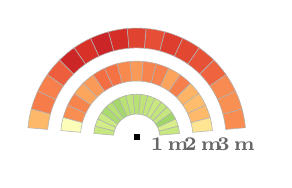
\begin{tikzpicture}[x=\fpscale cm, y=\fpscale cm, baseline=(current bounding box.north)]
  \fill[fill={rgb,1:red,0.7187;green,0.8801;blue,0.4597}, draw=black!30, line width=0.2pt] (95.0:0.7) arc[start angle=95.0, end angle=85.0, radius=0.7] -- (85.0:1.3) arc[start angle=85.0, end angle=95.0, radius=1.3] -- cycle;
  \fill[fill={rgb,1:red,0.7505;green,0.8938;blue,0.4802}, draw=black!30, line width=0.2pt] (105.0:0.7) arc[start angle=105.0, end angle=95.0, radius=0.7] -- (95.0:1.3) arc[start angle=95.0, end angle=105.0, radius=1.3] -- cycle;
  \fill[fill={rgb,1:red,0.7251;green,0.8829;blue,0.4638}, draw=black!30, line width=0.2pt] (115.0:0.7) arc[start angle=115.0, end angle=105.0, radius=0.7] -- (105.0:1.3) arc[start angle=105.0, end angle=115.0, radius=1.3] -- cycle;
  \fill[fill={rgb,1:red,0.6427;green,0.8474;blue,0.4151}, draw=black!30, line width=0.2pt] (125.0:0.7) arc[start angle=125.0, end angle=115.0, radius=0.7] -- (115.0:1.3) arc[start angle=115.0, end angle=125.0, radius=1.3] -- cycle;
  \fill[fill={rgb,1:red,0.7122;green,0.8773;blue,0.4555}, draw=black!30, line width=0.2pt] (135.0:0.7) arc[start angle=135.0, end angle=125.0, radius=0.7] -- (125.0:1.3) arc[start angle=125.0, end angle=135.0, radius=1.3] -- cycle;
  \fill[fill={rgb,1:red,0.6664;green,0.8576;blue,0.4259}, draw=black!30, line width=0.2pt] (145.0:0.7) arc[start angle=145.0, end angle=135.0, radius=0.7] -- (135.0:1.3) arc[start angle=135.0, end angle=145.0, radius=1.3] -- cycle;
  \fill[fill={rgb,1:red,0.7929;green,0.912;blue,0.5075}, draw=black!30, line width=0.2pt] (155.0:0.7) arc[start angle=155.0, end angle=145.0, radius=0.7] -- (145.0:1.3) arc[start angle=145.0, end angle=155.0, radius=1.3] -- cycle;
  \fill[fill={rgb,1:red,0.8222;green,0.9246;blue,0.5264}, draw=black!30, line width=0.2pt] (165.0:0.7) arc[start angle=165.0, end angle=155.0, radius=0.7] -- (155.0:1.3) arc[start angle=155.0, end angle=165.0, radius=1.3] -- cycle;
  \fill[fill={rgb,1:red,0.7755;green,0.9045;blue,0.4963}, draw=black!30, line width=0.2pt] (175.0:0.7) arc[start angle=175.0, end angle=165.0, radius=0.7] -- (165.0:1.3) arc[start angle=165.0, end angle=175.0, radius=1.3] -- cycle;
  \fill[fill={rgb,1:red,0.7427;green,0.8905;blue,0.4752}, draw=black!30, line width=0.2pt] (85.0:0.7) arc[start angle=85.0, end angle=75.0, radius=0.7] -- (75.0:1.3) arc[start angle=75.0, end angle=85.0, radius=1.3] -- cycle;
  \fill[fill={rgb,1:red,0.762;green,0.8987;blue,0.4876}, draw=black!30, line width=0.2pt] (75.0:0.7) arc[start angle=75.0, end angle=65.0, radius=0.7] -- (65.0:1.3) arc[start angle=65.0, end angle=75.0, radius=1.3] -- cycle;
  \fill[fill={rgb,1:red,0.7908;green,0.9111;blue,0.5062}, draw=black!30, line width=0.2pt] (65.0:0.7) arc[start angle=65.0, end angle=55.0, radius=0.7] -- (55.0:1.3) arc[start angle=55.0, end angle=65.0, radius=1.3] -- cycle;
  \fill[fill={rgb,1:red,0.7605;green,0.8981;blue,0.4866}, draw=black!30, line width=0.2pt] (55.0:0.7) arc[start angle=55.0, end angle=45.0, radius=0.7] -- (45.0:1.3) arc[start angle=45.0, end angle=55.0, radius=1.3] -- cycle;
  \fill[fill={rgb,1:red,0.7723;green,0.9031;blue,0.4942}, draw=black!30, line width=0.2pt] (45.0:0.7) arc[start angle=45.0, end angle=35.0, radius=0.7] -- (35.0:1.3) arc[start angle=35.0, end angle=45.0, radius=1.3] -- cycle;
  \fill[fill={rgb,1:red,0.6239;green,0.8391;blue,0.413}, draw=black!30, line width=0.2pt] (35.0:0.7) arc[start angle=35.0, end angle=25.0, radius=0.7] -- (25.0:1.3) arc[start angle=25.0, end angle=35.0, radius=1.3] -- cycle;
  \fill[fill={rgb,1:red,0.8469;green,0.9353;blue,0.5424}, draw=black!30, line width=0.2pt] (25.0:0.7) arc[start angle=25.0, end angle=15.0, radius=0.7] -- (15.0:1.3) arc[start angle=15.0, end angle=25.0, radius=1.3] -- cycle;
  \fill[fill={rgb,1:red,0.7815;green,0.9071;blue,0.5002}, draw=black!30, line width=0.2pt] (15.0:0.7) arc[start angle=15.0, end angle=5.0, radius=0.7] -- (5.0:1.3) arc[start angle=5.0, end angle=15.0, radius=1.3] -- cycle;
  \fill[fill={rgb,1:red,0.9813;green,0.6041;blue,0.3443}, draw=black!30, line width=0.2pt] (95.0:1.7) arc[start angle=95.0, end angle=85.0, radius=1.7] -- (85.0:2.3) arc[start angle=85.0, end angle=95.0, radius=2.3] -- cycle;
  \fill[fill={rgb,1:red,0.9725;green,0.5398;blue,0.3147}, draw=black!30, line width=0.2pt] (105.0:1.7) arc[start angle=105.0, end angle=95.0, radius=1.7] -- (95.0:2.3) arc[start angle=95.0, end angle=105.0, radius=2.3] -- cycle;
  \fill[fill={rgb,1:red,0.9598;green,0.4472;blue,0.2723}, draw=black!30, line width=0.2pt] (115.0:1.7) arc[start angle=115.0, end angle=105.0, radius=1.7] -- (105.0:2.3) arc[start angle=105.0, end angle=115.0, radius=2.3] -- cycle;
  \fill[fill={rgb,1:red,0.9574;green,0.4301;blue,0.2644}, draw=black!30, line width=0.2pt] (125.0:1.7) arc[start angle=125.0, end angle=115.0, radius=1.7] -- (115.0:2.3) arc[start angle=115.0, end angle=125.0, radius=2.3] -- cycle;
  \fill[fill={rgb,1:red,0.9812;green,0.6032;blue,0.3438}, draw=black!30, line width=0.2pt] (135.0:1.7) arc[start angle=135.0, end angle=125.0, radius=1.7] -- (125.0:2.3) arc[start angle=125.0, end angle=135.0, radius=2.3] -- cycle;
  \fill[fill={rgb,1:red,0.9872;green,0.6469;blue,0.3639}, draw=black!30, line width=0.2pt] (145.0:1.7) arc[start angle=145.0, end angle=135.0, radius=1.7] -- (135.0:2.3) arc[start angle=135.0, end angle=145.0, radius=2.3] -- cycle;
  \fill[fill={rgb,1:red,0.9691;green,0.5153;blue,0.3035}, draw=black!30, line width=0.2pt] (155.0:1.7) arc[start angle=155.0, end angle=145.0, radius=1.7] -- (145.0:2.3) arc[start angle=145.0, end angle=155.0, radius=2.3] -- cycle;
  \fill[fill={rgb,1:red,0.975;green,0.5582;blue,0.3232}, draw=black!30, line width=0.2pt] (165.0:1.7) arc[start angle=165.0, end angle=155.0, radius=1.7] -- (155.0:2.3) arc[start angle=155.0, end angle=165.0, radius=2.3] -- cycle;
  \fill[fill={rgb,1:red,0.983;green,0.9928;blue,0.7257}, draw=black!30, line width=0.2pt] (175.0:1.7) arc[start angle=175.0, end angle=165.0, radius=1.7] -- (165.0:2.3) arc[start angle=165.0, end angle=175.0, radius=2.3] -- cycle;
  \fill[fill={rgb,1:red,0.9695;green,0.518;blue,0.3047}, draw=black!30, line width=0.2pt] (85.0:1.7) arc[start angle=85.0, end angle=75.0, radius=1.7] -- (75.0:2.3) arc[start angle=75.0, end angle=85.0, radius=2.3] -- cycle;
  \fill[fill={rgb,1:red,0.9686;green,0.5116;blue,0.3018}, draw=black!30, line width=0.2pt] (75.0:1.7) arc[start angle=75.0, end angle=65.0, radius=1.7] -- (65.0:2.3) arc[start angle=65.0, end angle=75.0, radius=2.3] -- cycle;
  \fill[fill={rgb,1:red,0.9864;green,0.6415;blue,0.3614}, draw=black!30, line width=0.2pt] (65.0:1.7) arc[start angle=65.0, end angle=55.0, radius=1.7] -- (55.0:2.3) arc[start angle=55.0, end angle=65.0, radius=2.3] -- cycle;
  \fill[fill={rgb,1:red,0.9669;green,0.4989;blue,0.296}, draw=black!30, line width=0.2pt] (55.0:1.7) arc[start angle=55.0, end angle=45.0, radius=1.7] -- (45.0:2.3) arc[start angle=45.0, end angle=55.0, radius=2.3] -- cycle;
  \fill[fill={rgb,1:red,0.9925;green,0.7069;blue,0.401}, draw=black!30, line width=0.2pt] (45.0:1.7) arc[start angle=45.0, end angle=35.0, radius=1.7] -- (35.0:2.3) arc[start angle=35.0, end angle=45.0, radius=2.3] -- cycle;
  \fill[fill={rgb,1:red,0.9932;green,0.74;blue,0.4288}, draw=black!30, line width=0.2pt] (35.0:1.7) arc[start angle=35.0, end angle=25.0, radius=1.7] -- (25.0:2.3) arc[start angle=25.0, end angle=35.0, radius=2.3] -- cycle;
  \fill[fill={rgb,1:red,0.993;green,0.7301;blue,0.4205}, draw=black!30, line width=0.2pt] (25.0:1.7) arc[start angle=25.0, end angle=15.0, radius=1.7] -- (15.0:2.3) arc[start angle=15.0, end angle=25.0, radius=2.3] -- cycle;
  \fill[fill={rgb,1:red,0.9967;green,0.899;blue,0.5801}, draw=black!30, line width=0.2pt] (15.0:1.7) arc[start angle=15.0, end angle=5.0, radius=1.7] -- (5.0:2.3) arc[start angle=5.0, end angle=15.0, radius=2.3] -- cycle;
  \fill[fill={rgb,1:red,0.8784;green,0.2623;blue,0.1872}, draw=black!30, line width=0.2pt] (95.0:2.7) arc[start angle=95.0, end angle=85.0, radius=2.7] -- (85.0:3.3) arc[start angle=85.0, end angle=95.0, radius=3.3] -- cycle;
  \fill[fill={rgb,1:red,0.8349;green,0.1802;blue,0.1528}, draw=black!30, line width=0.2pt] (105.0:2.7) arc[start angle=105.0, end angle=95.0, radius=2.7] -- (95.0:3.3) arc[start angle=95.0, end angle=105.0, radius=3.3] -- cycle;
  \fill[fill={rgb,1:red,0.7997;green,0.1464;blue,0.1521}, draw=black!30, line width=0.2pt] (115.0:2.7) arc[start angle=115.0, end angle=105.0, radius=2.7] -- (105.0:3.3) arc[start angle=105.0, end angle=115.0, radius=3.3] -- cycle;
  \fill[fill={rgb,1:red,0.8462;green,0.1946;blue,0.156}, draw=black!30, line width=0.2pt] (125.0:2.7) arc[start angle=125.0, end angle=115.0, radius=2.7] -- (115.0:3.3) arc[start angle=115.0, end angle=125.0, radius=3.3] -- cycle;
  \fill[fill={rgb,1:red,0.8039;green,0.1505;blue,0.1522}, draw=black!30, line width=0.2pt] (135.0:2.7) arc[start angle=135.0, end angle=125.0, radius=2.7] -- (125.0:3.3) arc[start angle=125.0, end angle=135.0, radius=3.3] -- cycle;
  \fill[fill={rgb,1:red,0.9301;green,0.3706;blue,0.2371}, draw=black!30, line width=0.2pt] (145.0:2.7) arc[start angle=145.0, end angle=135.0, radius=2.7] -- (135.0:3.3) arc[start angle=135.0, end angle=145.0, radius=3.3] -- cycle;
  \fill[fill={rgb,1:red,0.9672;green,0.5013;blue,0.2971}, draw=black!30, line width=0.2pt] (155.0:2.7) arc[start angle=155.0, end angle=145.0, radius=2.7] -- (145.0:3.3) arc[start angle=145.0, end angle=155.0, radius=3.3] -- cycle;
  \fill[fill={rgb,1:red,0.965;green,0.4854;blue,0.2898}, draw=black!30, line width=0.2pt] (165.0:2.7) arc[start angle=165.0, end angle=155.0, radius=2.7] -- (155.0:3.3) arc[start angle=155.0, end angle=165.0, radius=3.3] -- cycle;
  \fill[fill={rgb,1:red,0.9928;green,0.7211;blue,0.4129}, draw=black!30, line width=0.2pt] (175.0:2.7) arc[start angle=175.0, end angle=165.0, radius=2.7] -- (165.0:3.3) arc[start angle=165.0, end angle=175.0, radius=3.3] -- cycle;
  \fill[fill={rgb,1:red,0.9004;green,0.3083;blue,0.2084}, draw=black!30, line width=0.2pt] (85.0:2.7) arc[start angle=85.0, end angle=75.0, radius=2.7] -- (75.0:3.3) arc[start angle=75.0, end angle=85.0, radius=3.3] -- cycle;
  \fill[fill={rgb,1:red,0.8695;green,0.2435;blue,0.1785}, draw=black!30, line width=0.2pt] (75.0:2.7) arc[start angle=75.0, end angle=65.0, radius=2.7] -- (65.0:3.3) arc[start angle=65.0, end angle=75.0, radius=3.3] -- cycle;
  \fill[fill={rgb,1:red,0.8852;green,0.2765;blue,0.1937}, draw=black!30, line width=0.2pt] (65.0:2.7) arc[start angle=65.0, end angle=55.0, radius=2.7] -- (55.0:3.3) arc[start angle=55.0, end angle=65.0, radius=3.3] -- cycle;
  \fill[fill={rgb,1:red,0.9063;green,0.3206;blue,0.214}, draw=black!30, line width=0.2pt] (55.0:2.7) arc[start angle=55.0, end angle=45.0, radius=2.7] -- (45.0:3.3) arc[start angle=45.0, end angle=55.0, radius=3.3] -- cycle;
  \fill[fill={rgb,1:red,0.939;green,0.3892;blue,0.2456}, draw=black!30, line width=0.2pt] (45.0:2.7) arc[start angle=45.0, end angle=35.0, radius=2.7] -- (35.0:3.3) arc[start angle=35.0, end angle=45.0, radius=3.3] -- cycle;
  \fill[fill={rgb,1:red,0.9734;green,0.5465;blue,0.3178}, draw=black!30, line width=0.2pt] (35.0:2.7) arc[start angle=35.0, end angle=25.0, radius=2.7] -- (25.0:3.3) arc[start angle=25.0, end angle=35.0, radius=3.3] -- cycle;
  \fill[fill={rgb,1:red,0.976;green,0.5653;blue,0.3264}, draw=black!30, line width=0.2pt] (25.0:2.7) arc[start angle=25.0, end angle=15.0, radius=2.7] -- (15.0:3.3) arc[start angle=15.0, end angle=25.0, radius=3.3] -- cycle;
  \fill[fill={rgb,1:red,0.9739;green,0.5503;blue,0.3196}, draw=black!30, line width=0.2pt] (15.0:2.7) arc[start angle=15.0, end angle=5.0, radius=2.7] -- (5.0:3.3) arc[start angle=5.0, end angle=15.0, radius=3.3] -- cycle;
  \fill[black] (-0.09, -0.09) rectangle (0.09, 0.09);
  \node[font=\scriptsize\bfseries, text=black!60] at (1, -0.22) {1\,m};
  \node[font=\scriptsize\bfseries, text=black!60] at (2, -0.22) {2\,m};
  \node[font=\scriptsize\bfseries, text=black!60] at (3, -0.22) {3\,m};
\end{tikzpicture}
 & % floorplan colorbar: trans — generated, edit freely
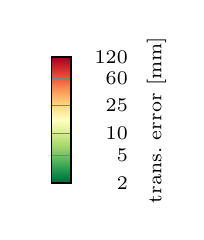
\begin{tikzpicture}[baseline=(current bounding box.north)]
\pgfplotsset{colormap={rdylgnrev}{rgb=(0.0,0.408,0.216) rgb=(0.0729,0.5423,0.286) rgb=(0.2297,0.6581,0.3457) rgb=(0.4359,0.7567,0.392) rgb=(0.6151,0.8353,0.412) rgb=(0.7653,0.9001,0.4897) rgb=(0.8936,0.955,0.6033) rgb=(1.0,1.0,0.749) rgb=(0.9971,0.9129,0.6033) rgb=(0.9943,0.794,0.4743) rgb=(0.987,0.6456,0.3633) rgb=(0.962,0.4634,0.2797) rgb=(0.8919,0.2904,0.2001) rgb=(0.787,0.1343,0.1519) rgb=(0.647,0.0,0.149)}, colormap={rdylgn}{rgb=(0.647,0.0,0.149) rgb=(0.787,0.1343,0.1519) rgb=(0.8919,0.2904,0.2001) rgb=(0.962,0.4634,0.2797) rgb=(0.987,0.6456,0.3633) rgb=(0.9943,0.794,0.4743) rgb=(0.9971,0.9129,0.6033) rgb=(1.0,1.0,0.749) rgb=(0.8936,0.955,0.6033) rgb=(0.7653,0.9001,0.4897) rgb=(0.6151,0.8353,0.412) rgb=(0.4359,0.7567,0.392) rgb=(0.2297,0.6581,0.3457) rgb=(0.0729,0.5423,0.286) rgb=(0.0,0.408,0.216)}}
\begin{axis}[hide axis, scale only axis, width=0pt, height=1.6cm,
  colormap name=rdylgnrev, colorbar, point meta min=0.301, point meta max=2.0792,
  colorbar style={height=1.6cm, width=0.25cm, ylabel={trans.~error [mm]}, ylabel style={font=\scriptsize},
    ytick={0.301,0.699,1.0,1.3979,1.7782,2.0792}, yticklabels={2,5,10,25,60,120}, tick label style={font=\scriptsize},
    yticklabel style={text width=1.7em, align=right}}]
  \addplot[draw=none] coordinates {(0,0)};
\end{axis}
\end{tikzpicture}
 \\[2pt]
\multicolumn{3}{c}{(b) Median Translation Error [mm]} & \\
\end{tabular}
